% Options for packages loaded elsewhere
\PassOptionsToPackage{unicode}{hyperref}
\PassOptionsToPackage{hyphens}{url}
\documentclass[
]{article}
\usepackage{xcolor}
\usepackage[margin=1in]{geometry}
\usepackage{amsmath,amssymb}
\setcounter{secnumdepth}{-\maxdimen} % remove section numbering
\usepackage{iftex}
\ifPDFTeX
  \usepackage[T1]{fontenc}
  \usepackage[utf8]{inputenc}
  \usepackage{textcomp} % provide euro and other symbols
\else % if luatex or xetex
  \usepackage{unicode-math} % this also loads fontspec
  \defaultfontfeatures{Scale=MatchLowercase}
  \defaultfontfeatures[\rmfamily]{Ligatures=TeX,Scale=1}
\fi
\usepackage{lmodern}
\ifPDFTeX\else
  % xetex/luatex font selection
\fi
% Use upquote if available, for straight quotes in verbatim environments
\IfFileExists{upquote.sty}{\usepackage{upquote}}{}
\IfFileExists{microtype.sty}{% use microtype if available
  \usepackage[]{microtype}
  \UseMicrotypeSet[protrusion]{basicmath} % disable protrusion for tt fonts
}{}
\makeatletter
\@ifundefined{KOMAClassName}{% if non-KOMA class
  \IfFileExists{parskip.sty}{%
    \usepackage{parskip}
  }{% else
    \setlength{\parindent}{0pt}
    \setlength{\parskip}{6pt plus 2pt minus 1pt}}
}{% if KOMA class
  \KOMAoptions{parskip=half}}
\makeatother
\usepackage{color}
\usepackage{fancyvrb}
\newcommand{\VerbBar}{|}
\newcommand{\VERB}{\Verb[commandchars=\\\{\}]}
\DefineVerbatimEnvironment{Highlighting}{Verbatim}{commandchars=\\\{\}}
% Add ',fontsize=\small' for more characters per line
\usepackage{framed}
\definecolor{shadecolor}{RGB}{248,248,248}
\newenvironment{Shaded}{\begin{snugshade}}{\end{snugshade}}
\newcommand{\AlertTok}[1]{\textcolor[rgb]{0.94,0.16,0.16}{#1}}
\newcommand{\AnnotationTok}[1]{\textcolor[rgb]{0.56,0.35,0.01}{\textbf{\textit{#1}}}}
\newcommand{\AttributeTok}[1]{\textcolor[rgb]{0.13,0.29,0.53}{#1}}
\newcommand{\BaseNTok}[1]{\textcolor[rgb]{0.00,0.00,0.81}{#1}}
\newcommand{\BuiltInTok}[1]{#1}
\newcommand{\CharTok}[1]{\textcolor[rgb]{0.31,0.60,0.02}{#1}}
\newcommand{\CommentTok}[1]{\textcolor[rgb]{0.56,0.35,0.01}{\textit{#1}}}
\newcommand{\CommentVarTok}[1]{\textcolor[rgb]{0.56,0.35,0.01}{\textbf{\textit{#1}}}}
\newcommand{\ConstantTok}[1]{\textcolor[rgb]{0.56,0.35,0.01}{#1}}
\newcommand{\ControlFlowTok}[1]{\textcolor[rgb]{0.13,0.29,0.53}{\textbf{#1}}}
\newcommand{\DataTypeTok}[1]{\textcolor[rgb]{0.13,0.29,0.53}{#1}}
\newcommand{\DecValTok}[1]{\textcolor[rgb]{0.00,0.00,0.81}{#1}}
\newcommand{\DocumentationTok}[1]{\textcolor[rgb]{0.56,0.35,0.01}{\textbf{\textit{#1}}}}
\newcommand{\ErrorTok}[1]{\textcolor[rgb]{0.64,0.00,0.00}{\textbf{#1}}}
\newcommand{\ExtensionTok}[1]{#1}
\newcommand{\FloatTok}[1]{\textcolor[rgb]{0.00,0.00,0.81}{#1}}
\newcommand{\FunctionTok}[1]{\textcolor[rgb]{0.13,0.29,0.53}{\textbf{#1}}}
\newcommand{\ImportTok}[1]{#1}
\newcommand{\InformationTok}[1]{\textcolor[rgb]{0.56,0.35,0.01}{\textbf{\textit{#1}}}}
\newcommand{\KeywordTok}[1]{\textcolor[rgb]{0.13,0.29,0.53}{\textbf{#1}}}
\newcommand{\NormalTok}[1]{#1}
\newcommand{\OperatorTok}[1]{\textcolor[rgb]{0.81,0.36,0.00}{\textbf{#1}}}
\newcommand{\OtherTok}[1]{\textcolor[rgb]{0.56,0.35,0.01}{#1}}
\newcommand{\PreprocessorTok}[1]{\textcolor[rgb]{0.56,0.35,0.01}{\textit{#1}}}
\newcommand{\RegionMarkerTok}[1]{#1}
\newcommand{\SpecialCharTok}[1]{\textcolor[rgb]{0.81,0.36,0.00}{\textbf{#1}}}
\newcommand{\SpecialStringTok}[1]{\textcolor[rgb]{0.31,0.60,0.02}{#1}}
\newcommand{\StringTok}[1]{\textcolor[rgb]{0.31,0.60,0.02}{#1}}
\newcommand{\VariableTok}[1]{\textcolor[rgb]{0.00,0.00,0.00}{#1}}
\newcommand{\VerbatimStringTok}[1]{\textcolor[rgb]{0.31,0.60,0.02}{#1}}
\newcommand{\WarningTok}[1]{\textcolor[rgb]{0.56,0.35,0.01}{\textbf{\textit{#1}}}}
\usepackage{longtable,booktabs,array}
\usepackage{calc} % for calculating minipage widths
% Correct order of tables after \paragraph or \subparagraph
\usepackage{etoolbox}
\makeatletter
\patchcmd\longtable{\par}{\if@noskipsec\mbox{}\fi\par}{}{}
\makeatother
% Allow footnotes in longtable head/foot
\IfFileExists{footnotehyper.sty}{\usepackage{footnotehyper}}{\usepackage{footnote}}
\makesavenoteenv{longtable}
\usepackage{graphicx}
\makeatletter
\newsavebox\pandoc@box
\newcommand*\pandocbounded[1]{% scales image to fit in text height/width
  \sbox\pandoc@box{#1}%
  \Gscale@div\@tempa{\textheight}{\dimexpr\ht\pandoc@box+\dp\pandoc@box\relax}%
  \Gscale@div\@tempb{\linewidth}{\wd\pandoc@box}%
  \ifdim\@tempb\p@<\@tempa\p@\let\@tempa\@tempb\fi% select the smaller of both
  \ifdim\@tempa\p@<\p@\scalebox{\@tempa}{\usebox\pandoc@box}%
  \else\usebox{\pandoc@box}%
  \fi%
}
% Set default figure placement to htbp
\def\fps@figure{htbp}
\makeatother
\setlength{\emergencystretch}{3em} % prevent overfull lines
\providecommand{\tightlist}{%
  \setlength{\itemsep}{0pt}\setlength{\parskip}{0pt}}
\usepackage{fontspec}
\setmainfont{DejaVu Serif}
\usepackage{booktabs}
\usepackage{longtable}
\usepackage{array}
\usepackage{multirow}
\usepackage{wrapfig}
\usepackage{float}
\usepackage{colortbl}
\usepackage{pdflscape}
\usepackage{tabu}
\usepackage{threeparttable}
\usepackage{threeparttablex}
\usepackage[normalem]{ulem}
\usepackage{makecell}
\usepackage{xcolor}
\usepackage{bookmark}
\IfFileExists{xurl.sty}{\usepackage{xurl}}{} % add URL line breaks if available
\urlstyle{same}
\hypersetup{
  pdftitle={Chapter 1: Counting Words in the 19th-Century British Parliamentary Debates},
  hidelinks,
  pdfcreator={LaTeX via pandoc}}

\title{Chapter 1: Counting Words in the 19th-Century British
Parliamentary Debates}
\author{}
\date{\vspace{-2.5em}}

\begin{document}
\maketitle

The introduction to text mining in this book begins with tracking words'
context by processing data, counting words, and visualizing the words
that co-occur with one-another. As the linguist John Rupert Firth (1974)
said, ``You shall know a word by the company it keeps.'' Tracking subtle
variations in the context with which different words are used helps
historians and other analysts to understand the cultural biases that
structure our collective thinking. They may help us to understand how a
culture understands men and women differently, how a culture describes
people of different nationalities, the difference between a concept like
``the foreign'' and its near synonyms like ``outsider'' that
nevertheless are used in important and different ways, or how these
concepts are changing over time. In the course of this book, we will
offer a taste of the subtle and refined approaches that analysts have
used to unpack the context of different words.

Understanding the historical context of language begins with how we
interpret and approach individual words. In this chapter, we treat the
words we process as ``keywords''--terms that are central to
understanding culture and society, but whose meanings are often
contested or have shifted over time (Williams 1985). For example, the
word ``labour'' may be a particularly interesting word to an analyst of
19th-century Britain, more so than the word ``table.'' This is because
in the 19th-century debates, the meaning of the word ``labour'' evolved
alongside industrialization, class conflict, and political reform. Early
in the century, labour was often used in economic terms, referring to
the input of human work in production, as discussed by political
economists like Adam Smith. But as the century progressed---and
especially with the rise of trade unions, Chartism, and later the Labour
movement---the term labour took on a more political and moral dimension.
It began to signify not just work, but the working class itself, with
connotations of exploitation, rights, and collective struggle. The
meaning of the word ``table'' on the other hand, is generally stable,
literal, and uncontroversial. It refers to a physical object--typically
a piece of furniture--and does not carry the kind of cultural
significance that keywords do.

Recognizing words as evolving and changing--rather than fixed--allows us
to glean greater insight into how language reflects broader cultural
transformations. It invites us not to take words at face value, but to
remember that language is dynamic and often shaped by power struggles,
and that the way we process data impacts our subsequent analyses of
these power struggles.

The data processing techniques we foreground will lead to our first
visualization, where we transform individual utterances or debates into
high-level visualizations depicting the frequencies of keywords and
their associations (Moretti 2013, Jockers 2013). To achieve this end, we
will introduce three basic techniques for processing text. We will: a)
access data for the British parliamentary debates of the House of Lords
and House of Commons, 1850-59 using the \texttt{hansardr} library, b)
filter a relevant decade for keywords of interest, and c) count the
words that appear in the same context as our keywords in order to study
the associations of the keywords in more detail.

Importantly, the techniques presented in this chapter have both promise
and limits. As our companion volume, \emph{The Dangerous Art of Text
Mining} (2023), makes clear, simple word counts are almost never
sufficient on their own to support an in-depth analysis of culture.
Nevertheless, knowing how to count words and compare the context with
which different concepts are used is a first step to using text as data.
Recognizing that langauge contains keywords that can, for example, be
chosen by an analyst to guide data processing is a first step towards
producing meaning from text data.

\subsection{Running a Line of Code}\label{running-a-line-of-code}

The first step in learning R is understanding how to run a line of code.

Here are some exercises to learn how to run code on your computer. Try
each and decide which ones feel most comfortable to you: - You can type
a command directly into the Console pane and press Enter. - You can
write it in an R script and execute it by placing your curser on the
line you want to run and press \texttt{Ctrl\ +\ Enter} on Windows or
Linux (or \texttt{Cmd\ +\ Enter} on a Mac). - You can also highlight one
or more lines of code and click the green Run button at the top of the
script editor.

Try to run the code now by typing the following into your Console and
pressing Enter, or by highlighting it and clicking Run:

\begin{Shaded}
\begin{Highlighting}[]
\FunctionTok{print}\NormalTok{(}\StringTok{"Hello World"}\NormalTok{)}
\end{Highlighting}
\end{Shaded}

\begin{verbatim}
## [1] "Hello World"
\end{verbatim}

This should display the phrase ``Hello World'' beneath your code,
confirming that R executed the command.

\subsection{Loading the Hansard Data}\label{loading-the-hansard-data}

First we will load the data we wish to analyze. Analysts, programmers,
researchers, and the like routinely import software packages developed
by others to expand the range of tools available to them.

The authors developed a data package to go with this book,
\texttt{hansardr}, to give readers an ability to access the Hansard
19th-Century British Parliamentary Debates within the R environment
(Buongiorno 2022). This is a cleaned, analysis-ready corpus of the
19th-century British Parliamentary Debates (1803-1899), also known as
``Hansard'' in reference to Thomas Curzon Hansard, the publisher. It
identifies debates whose records are missing from UK Parliament's
corpus, and it also offers a field for disambiguated speakers. We
believe this dataset will enable researchers to analyze the Hansard
debates, including speaker discourse, in a way that has not been
accessible before. Once installed, the data can be loaded with the
\texttt{data()} function.

Functions are an important characteristic of the R language. Unlike
other popular programming languages--such as Python--R is a functional
language, which means it emphasizes processing data using these
functions rather than relying on complex programming syntax. In R, a
function is a block of code that performs a specific task. It can take
inputs, called ``arguments'', that serve as instructions for how the
function should behave, process data, or return an output. Functions are
like the verbs of the R language in the sense that they say what should
be done to the data. We will use functions throughout this book to
perform data processing.

To use a function from another package, you must first install the
package with \texttt{install.packages().} Here is how you would install
the packages used in this chapter with \texttt{install.packages()}
before loading them with \texttt{library()}, which we demonstrate later
in the chapter:

\begin{Shaded}
\begin{Highlighting}[]
\FunctionTok{install.packages}\NormalTok{(}\StringTok{"tidyverse"}\NormalTok{)}
\end{Highlighting}
\end{Shaded}

\begin{verbatim}
## Installing package into '/home/stephbuongiorno/R/x86_64-pc-linux-gnu-library/4.5'
## (as 'lib' is unspecified)
\end{verbatim}

\begin{Shaded}
\begin{Highlighting}[]
\FunctionTok{install.packages}\NormalTok{(}\StringTok{"tidytext"}\NormalTok{)}
\end{Highlighting}
\end{Shaded}

\begin{verbatim}
## Installing package into '/home/stephbuongiorno/R/x86_64-pc-linux-gnu-library/4.5'
## (as 'lib' is unspecified)
\end{verbatim}

\begin{Shaded}
\begin{Highlighting}[]
\FunctionTok{install.packages}\NormalTok{(}\StringTok{"quanteda"}\NormalTok{)}
\end{Highlighting}
\end{Shaded}

\begin{verbatim}
## Installing package into '/home/stephbuongiorno/R/x86_64-pc-linux-gnu-library/4.5'
## (as 'lib' is unspecified)
\end{verbatim}

In RStudio, you can also verify whether a package is already installed
by checking the Packages tab in the lower-right panel. This tab displays
all packages currently available in your R library. If a package appears
in that list, it is already installed; if not, you can install it using
\texttt{install.packages()}. You can also load an installed package by
checking the box next to its name in this tab, which is equivalent to
calling \texttt{library()} in your script.

When installing code or data from a repository such as GitHub, we can
use a special installation script that we created for this book.

If RStudio prompts you to restart R while installing a package, click
Yes to allow the restart, and then re-run the installation command so
the package loads into the fresh session.

\begin{Shaded}
\begin{Highlighting}[]
\FunctionTok{source}\NormalTok{(}\StringTok{"https://raw.githubusercontent.com/Democracy{-}Lab/hansardr/master/tools/install\_hansardr.R"}\NormalTok{)}
\end{Highlighting}
\end{Shaded}

As we explained in the introduction, packages only have to be installed
once, but they need to be reloaded for each new R session using
\texttt{library()}. Only once we have run \texttt{library(hansardr)}
will the data be available for our use.

\begin{Shaded}
\begin{Highlighting}[]
\CommentTok{\# load the hansardr package}
\FunctionTok{library}\NormalTok{(hansardr)}
\end{Highlighting}
\end{Shaded}

\texttt{hansardr} is now ready for use. It is conventional to load the
software packages that will be use at the beginning of each new session.
However, for the sake of demonstrating computational historical
thinking, we will regularly load packages throughout a chapter so the
reader can more easily see which functions relate back to different
packages.

When working with functions in R, it is important to remember that code
must be run in order, because each step often depends on what came
before it. For example, if we plan to use a package such as hansardr, we
must first load it with \texttt{library(hansardr)} before calling any of
its functions. If we skip this step, R will not know where the hansardr
functions come from and will return an error such as ``could not find
function,'' even if the code is correct. Similar errors can also occur
when data is not processed in the proper sequence, since later steps may
rely on datasets or data transformations that have not yet been created.

\subsubsection{\texorpdfstring{Navigating the \texttt{hansardr}
Data}{Navigating the hansardr Data}}\label{navigating-the-hansardr-data}

To make working with the Hansard corpus quicker and easier--and to
prevent our personal computers from being overloaded with too much data
at once--we partitioned the century long corpus into decade sections. In
the field of data analysis, it is common to call these sections
``subsets.''

The first subset we will meet is a collection of the speeches of
parliament, 1850-59, broken into sentences, where each row of the data
frame is one sentence. Later, we will meet more datasets that contain
``metadata,'' or information about the speaker, year and date of the
speech, and other important contextual information for historical
analysis.

The \texttt{hansardr} corpus is subsetted by decade. As shown by Table
1, each decade has four types of data, labeled: ``hansard,''
``debate\_metadata,'' ``speaker\_metadata,'' and ``file\_metadata.'' In
the following table, ``YYYY'' stands in for any given decade.

\begin{verbatim}
## -- Attaching core tidyverse packages ------------------------ tidyverse 2.0.0 --
## v dplyr     1.1.4     v readr     2.1.5
## v forcats   1.0.1     v stringr   1.5.2
## v ggplot2   4.0.0     v tibble    3.3.0
## v lubridate 1.9.4     v tidyr     1.3.1
## v purrr     1.1.0     
## -- Conflicts ------------------------------------------ tidyverse_conflicts() --
## x dplyr::filter()     masks stats::filter()
## x dplyr::group_rows() masks kableExtra::group_rows()
## x dplyr::lag()        masks stats::lag()
## i Use the conflicted package (<http://conflicted.r-lib.org/>) to force all conflicts to become errors
\end{verbatim}

\begin{longtable}[]{@{}
  >{\raggedright\arraybackslash}p{(\linewidth - 4\tabcolsep) * \real{0.2821}}
  >{\raggedright\arraybackslash}p{(\linewidth - 4\tabcolsep) * \real{0.5641}}
  >{\raggedright\arraybackslash}p{(\linewidth - 4\tabcolsep) * \real{0.1538}}@{}}
\caption{Table 1: Description of Hansard Corpus Files by
Decade}\tabularnewline
\toprule\noalign{}
\begin{minipage}[b]{\linewidth}\raggedright
Label
\end{minipage} & \begin{minipage}[b]{\linewidth}\raggedright
Description
\end{minipage} & \begin{minipage}[b]{\linewidth}\raggedright
Key
\end{minipage} \\
\midrule\noalign{}
\endfirsthead
\toprule\noalign{}
\begin{minipage}[b]{\linewidth}\raggedright
Label
\end{minipage} & \begin{minipage}[b]{\linewidth}\raggedright
Description
\end{minipage} & \begin{minipage}[b]{\linewidth}\raggedright
Key
\end{minipage} \\
\midrule\noalign{}
\endhead
\bottomrule\noalign{}
\endlastfoot
hansard\_YYYY & Hansard debate text & sentence\_id \\
debate\_metadata\_YYYY & Metadata such as speech date and title. &
sentence\_id \\
speaker\_metadata\_YYYY & Metadata on speakers. & sentence\_id \\
file\_metadata\_YYYY & Metadata for source file, column, and more. &
sentence\_id \\
\end{longtable}

Both text and metadata are divided into subsets named by decade, for
instance, \texttt{hansard\_1850}. \texttt{hansard\_1850} contains just
the speech text as well as a unique sentence ID that can be used to
connect the speech text with its corresponding metadata. We will
demonstrate this process later in \emph{Text Mining for Historical
Analysis}.

Processing both text and dates is important for historical analysis. In
this chapter, we will start working exclusively with text--not
dates--because they are easy to process when counting words. But the
other subsets within \texttt{hansardr} contain other data types.

We can use \texttt{data()} to load one of these decade-based subsets of
the Hansard corpus.

\begin{Shaded}
\begin{Highlighting}[]
\CommentTok{\# load the Hansard debate text for 1850}
\FunctionTok{data}\NormalTok{(}\StringTok{"hansard\_1850"}\NormalTok{)}
\end{Highlighting}
\end{Shaded}

A new variable named \texttt{hansard\_1850} is now able to be seen in
our Global Environment panel. If you are using RStudio, you can explore
the data by clicking on its name in the Global Environment pane (the top
right quadrant of RStudio). Clicking on the name of the dataset will
open a new tab containing a view of the data, which can be searched for
a keyword, like in a spreadsheet. One can also double-click on any row
in the data frame to select a row, then copy that data and paste it into
a Word Document or other tool.

The Hansard subsets are purposefully small enough to open and explore on
a personal computer. When working with larger datasets, it may not be
possible to open the entire dataset in another tab. Instead, in the
Global Environment Panel you can also click on the blue
``\textgreater{}'' symbol to the left of each data frame to display the
``fields'' by which the dataset is structured, in this case, the names
of the columns in the dataset, as well as a preview of the content of
each of these columns.

In addition to exploring the data in RStudio, there are a few functions
that provide the means to look at sections of the dataset in greater
detail. Throughout this book, we will routinely ``inspect'' the data by
using functions like \texttt{head()} to see how the data is transformed
at different processing steps. Getting into the habit of using functions
like \texttt{head()} makes it easier to notice and interrogate problems
as they arise, or ensure that the data transformations meet
expectations. At the console, an analyst can also use \texttt{head()} to
ask R to display the first six rows of the data. In some versions of
RStudio you will see an arrow that allows you to move between two
columns.

As shown by Table 2, the first column in this dataset is
\texttt{sentence\_id}, which gives a unique identifier for each
sentence, including information about which series of parliamentary
proceedings we are looking at, which volume and page, and which sentence
number on each page. The second column is \texttt{text}. Each row is a
distinct sentence of text. These speeches were broken into sentences
during the dataset creation stage, where the authors wrote a script to
detect punctuation and line breaks.

Below is an excerpt from \texttt{hansardr}:

\begin{table}
\centering
\caption{\label{tab:unnamed-chunk-6}Excerpt from Hansard 1850}
\centering
\resizebox{\ifdim\width>\linewidth\linewidth\else\width\fi}{!}{
\begin{tabular}[t]{lp{12cm}}
\toprule
sentence\_id & text\\
\midrule
\cellcolor{gray!10}{S3V0108P0\_0} & \cellcolor{gray!10}{, which had been prorogued successively from the 1st of August to the 9th of October, from thence to the 20th of November, thence to the 16th of January, and from thence to the 31st January, met this day for despatch of business.}\\
S3V0108P0\_1 & The Parliament was opened by Commission, the LORDS COMMISSIONERS present being the LORD CHANCELLOR; the LORD PRESIDENT OF THE COUNCIL (the Marquess of Lansdowne); the LORD PRIVY SEAL (the Earl of Minto); the LORD CHAMBERLAIN OF THE HOUSEHOLD (the Marquess of Breadalbane); and the LORD BISHOP OF LONDON.\\
\cellcolor{gray!10}{S3V0108P0\_2} & \cellcolor{gray!10}{called attention to a great omission of their duty on the part of Ministers, with respect to the privileges of their Lordships, which might and ought to have been avoided.}\\
S3V0108P0\_3 & At pre-sent there were two vacancies in the representative Peers of Scotland, in consequence of the deaths of the Earl of Airlie and of Lord Colville.\\
\cellcolor{gray!10}{S3V0108P0\_4} & \cellcolor{gray!10}{Although the Act of Parliament directed that the proclamation should issue forthwith for the election of representative Peers to fill up any vacancies which might occur, by death or otherwise, no such proclamation had yet taken place in the case of the two vacancies he had just mentioned, and the consequence was, that for twenty-four days after the meeting of Parliament it was not possible for any Scotch representative Peers to be elected.}\\
\bottomrule
\end{tabular}}
\end{table}

\subsection{Tidy Text Mining and Loading
Libraries}\label{tidy-text-mining-and-loading-libraries}

Most of the functions used in the first chapters of this book come from
a software package called \texttt{tidyverse} (2019) which is a family of
smaller packages developed by Chief Scientist at Posit (formerly known
as RStudio), Hadley Wickham.

The tidyverse was created to order data in ``tidy'' tables where it is
structured as a data frame made up of columns and rows. In other words,
the tidyverse is built to work with data like \texttt{hansard\_1850}.

We have found that a tidy approach to text exploration and analysis
allows us to write code quickly and effectively, giving us ample control
over the data and allowing us to inspect the output of every data
processing step and type of analysis. This library thus supports
analysts focusing on questions about data processing and history without
being weighed down by the nuances of different structural and syntactic
coding problems.

We distinguish between writing code and processing data, proposing that
data processing and historical analysis are co-creative practices. Data
processing shapes how we interpret the past---it is not a neutral task,
but one that governs the possibilities of historical understanding. At
the same time, the historical material we study--the observations we
make--might inform and reshape our data processing methods. We will
return to this central idea of ``computational historical
thinking''--which we introduce in our introduction--throughout the book,
as we demonstrate how iterative adjustments to our processing approach
impact our analysis.

In this chapter we will also use the \texttt{tidytext} library,
developed by David Robinson and Julia Silge (2016), to work with textual
data. The \texttt{tidytext} library contains a variety of tools useful
for processing text and treating text as data. Many sections in this
book will therefore begin by loading the two libraries
\texttt{tidyverse} and \texttt{tidytext}.

\begin{Shaded}
\begin{Highlighting}[]
\CommentTok{\# load the tidyverse and tidytext packages}
\FunctionTok{library}\NormalTok{(tidyverse)}
\FunctionTok{library}\NormalTok{(tidytext)}
\end{Highlighting}
\end{Shaded}

\subsection{Using Functions to Process
Data}\label{using-functions-to-process-data}

The primary purpose of a function is to create reusable code, allowing
analysts to avoid repeating the same data processing steps over and
over.

From this point on we are going to use more complicated functions from
different R packages to process our data. Before we take this next step,
however, we first want to provide a basic understanding of a function's
underlying components, by creating our own simple function:

\begin{Shaded}
\begin{Highlighting}[]
\CommentTok{\# define a custom function to add two numbers}
\NormalTok{add\_numbers }\OtherTok{\textless{}{-}} \ControlFlowTok{function}\NormalTok{(a, b) \{ }
\NormalTok{  result }\OtherTok{\textless{}{-}}\NormalTok{ a }\SpecialCharTok{+}\NormalTok{ b }
  \FunctionTok{return}\NormalTok{(result) \}}
\end{Highlighting}
\end{Shaded}

The above code can be broken down into these core parts:

\begin{enumerate}
\def\labelenumi{\arabic{enumi}.}
\tightlist
\item
  Function Name: The name given to the function. In this example, the
  function is named \texttt{add\_numbers}.
\item
  Parameters: The variables listed in the function definition that will
  accept arguments, for instance, \texttt{function(a,\ b)}.
\item
  Body: The code that is executed when the function is called, written
  here as \texttt{result\ \textless{}-\ a\ +\ b}.
\item
  Return Value: The output produced by the function, for example,
  \texttt{return(result)}.
\end{enumerate}

Every function in R encapsulates a code body, even when it is hidden
from the analyst.

We can now use our new \texttt{add\_numbers()} function by passing
arguments to the specified parameters. In this example, the ``a''
parameter is passed the number 2, and the ``b'' parameter is passed the
number 3. The two numbers are added in the body, and then the results
are returned.

Now that we have defined this function, we can call upon it whenever we
need to add two numbers without rewriting the steps involved. This kind
of reuse becomes especially important in historical analysis, which is
often iterative and rarely linear. As our interpretations shift and our
questions evolve, we often return to the same operations with new
purposes. Having stable tools like functions allows us to revisit and
revise our analyses without starting from scratch each time.

\begin{Shaded}
\begin{Highlighting}[]
\CommentTok{\# use the new function we created to add 2 and 3}
\FunctionTok{print}\NormalTok{(}\FunctionTok{add\_numbers}\NormalTok{(}\DecValTok{2}\NormalTok{, }\DecValTok{3}\NormalTok{))}
\end{Highlighting}
\end{Shaded}

\begin{verbatim}
## [1] 5
\end{verbatim}

To count words in Hansard, we will use a different function, the
\texttt{unnest\_tokens()} function from \texttt{tidytext}. While there
are many ways to count words over time, one way to do this--that is also
very human readable--is to put our data into a format where each word of
the text is on a separate row. These individual words are called
``tokens.'' The process of splitting chunks of text into individual
units is called ``tokenization.'' While singular words are often called
``tokens,'' a common term used to instead describe multi-word phrases is
``n-gram'' (such as using the term ``bigrams'' to describe sequential,
two-word phrases).

In this one-token-per-row format we can easily process our data. This
approach to data processing is common in the humanities and handles text
using the ``Bags of Words'' (BoW) approach, where text data is treated
as a collection (or ``bag'') of individual words without regard to
grammar, order, or context (Jockers 2015). The focus is instead on word
frequency or occurrence.

\begin{Shaded}
\begin{Highlighting}[]
\CommentTok{\# tokenize the \textquotesingle{}text\textquotesingle{} column of the hansard\_1850 dataset into individual words}
\CommentTok{\# {-} \textquotesingle{}unnest\_tokens()\textquotesingle{} from the \textquotesingle{}tidytext\textquotesingle{} package splits text into lowercase words}
\CommentTok{\# {-} the new column will be called \textquotesingle{}word\textquotesingle{}}
\CommentTok{\# {-} each word becomes its own row }
\NormalTok{tokenized\_hansard }\OtherTok{\textless{}{-}}\NormalTok{ hansard\_1850 }\SpecialCharTok{\%\textgreater{}\%} \CommentTok{\# create a new dataframe}
  \FunctionTok{unnest\_tokens}\NormalTok{(word, text) }\CommentTok{\# tokenize the \textquotesingle{}text\textquotesingle{} column }
\end{Highlighting}
\end{Shaded}

The above code also has new symbols, called ``operators.'' Operators are
essential for data processing. Throughout the course of this book we
will introduce multiple different kinds of operators.

The assignment operator, \texttt{\textless{}-}, sometimes translated as
``gets,'' points to the output of a function and is followed by the name
of an original dataset. The \texttt{\%\textgreater{}\%} operator, called
a ``pipe,'' and translated as ``next,'' is used to chain together
successive transformations of a dataset. This will make more sense when
we cover more examples later in the book.

If this is your first time using a programming language for analysis, it
can be useful to practice reading each line of code as a sentence of
instructions that tells the computer what output to make, what input to
use, and what processes to go through in a certain order. We sometimes
suggest that first time programmers translate code into a series of
English sentences, using their knowledge of the \texttt{\textless{}-}
and \texttt{\%\textgreater{}\%} operators, the names of variables, and
their understanding of distinct commands. The code above be read as
follows: ``Create a new variable called \texttt{tokenized\_hansard}.
Start with the dataset \texttt{hansard\_1850}. Next, unnest the tokens
in the''text'' column of \texttt{hansard\_1850}, unpacking those strings
of text into individual words.''

One may also notice the arguments passed to \texttt{unnest\_tokens()},
``word'' and ``text.'' Functions like \texttt{unnest\_tokens()} take a
set number of arguments, typically in a precise order. The first
argument is the type of unnesting that will be employed. The second
argument is the name of the column from the original
\texttt{hansard\_1850} data that we will work on, in this case,
``text.''

As you inspect the arguments of each function, consider the fact that
those arguments exist because they allow the analyst to change the
arguments to get different results. With the \texttt{unnest\_tokens()}
function, the analyst could hypothetically choose to ``unnest'' the
sentences into tokens of different length, for instance, sentences,
n-grams, or other units of text. In later chapters we will explore some
of these capabilities of the \texttt{unnest\_tokens()} function.
Alternatively, if \texttt{unnest\_tokens()} were being applied to a
different dataset where the column had a different name than ``text,''
we could change the column name from ``text'' to something else. In
later examples, we will use the same commands applied to different
datasets with different column names. For now, we will mainly use
\texttt{unnest\_tokens()} with the arguments ``word'' and ``text.''

Next, let's inspect the results of our unnesting using \texttt{head()},
which returns just the first rows of a data frame.

\begin{Shaded}
\begin{Highlighting}[]
\CommentTok{\# show the first few rows of our tokenized data}
\FunctionTok{head}\NormalTok{(tokenized\_hansard)}
\end{Highlighting}
\end{Shaded}

\begin{verbatim}
##   sentence_id         word
## 1 S3V0108P0_0        which
## 2 S3V0108P0_0          had
## 3 S3V0108P0_0         been
## 4 S3V0108P0_0    prorogued
## 5 S3V0108P0_0 successively
## 6 S3V0108P0_0         from
\end{verbatim}

However, we have a preference for looking at more data since that can
give us a fuller picture of the data.

\begin{Shaded}
\begin{Highlighting}[]
\CommentTok{\# show the first fifteen rows of our tokenized data}
\FunctionTok{head}\NormalTok{(tokenized\_hansard, }\AttributeTok{n=}\DecValTok{15}\NormalTok{)}
\end{Highlighting}
\end{Shaded}

\begin{verbatim}
##    sentence_id         word
## 1  S3V0108P0_0        which
## 2  S3V0108P0_0          had
## 3  S3V0108P0_0         been
## 4  S3V0108P0_0    prorogued
## 5  S3V0108P0_0 successively
## 6  S3V0108P0_0         from
## 7  S3V0108P0_0          the
## 8  S3V0108P0_0          1st
## 9  S3V0108P0_0           of
## 10 S3V0108P0_0       august
## 11 S3V0108P0_0           to
## 12 S3V0108P0_0          the
## 13 S3V0108P0_0          9th
## 14 S3V0108P0_0           of
## 15 S3V0108P0_0      october
\end{verbatim}

\texttt{unnest\_tokens()} did a lot of heavy lifting for us!

As part of our data transformation, the output data has a column named
``word'' for each individual token of the corpus. Notice that the words
in \texttt{tokenized\_hansard} look just like the words in the first
sentence of the first speech in \texttt{hansard\_1850}. Those speeches
have been split into individual words, but the words are still in the
same order. Notice that the command \texttt{unnest\_tokens()} has also
transformed all the words to lower-case and removed punctuation marks
such as commas and periods. This transformation, often called ``data
cleaning'' will make the words easier to count because the computer will
not treat words differently based on capitalization or the presence of
symbols.

As we inspect the results of unnesting, one might note that the input to
\texttt{unnest\_tokens()} was ``tidy'' in format -- that is, it had two
columns, one for ``sentence\_id'' and one for ``text''. After working
with \texttt{unnest\_tokens()}, the resulting output,
\texttt{tokenized\_hansard}, also is ``tidy'' in format. That is, it has
two columns, one for \texttt{sentence\_id} and one for \texttt{word}.
This tidy format is both easily human readable and also easy to process
and count.

\subsection{Counting Words}\label{counting-words}

Now we are going to bring together what we have learned by chaining
together multiple functions that will be used to process the Hansard
data.

The \texttt{count()} function from the \texttt{tidyverse} groups like
tokens with like tokens, then counts them. Below, we are passing
\texttt{count()} one argument, the name of the column to operate on--in
this case, ``word'' from the tokenized hansard data.

\begin{Shaded}
\begin{Highlighting}[]
\CommentTok{\# count the frequency of each word in the tokenized dataset}
\CommentTok{\# this creates a data frame with one row per unique word and a column \textquotesingle{}n\textquotesingle{} for the count}
\NormalTok{tokenized\_hansard\_counts }\OtherTok{\textless{}{-}}\NormalTok{ tokenized\_hansard }\SpecialCharTok{\%\textgreater{}\%} \CommentTok{\# Create a new data frame }
  \FunctionTok{count}\NormalTok{(word) }\SpecialCharTok{\%\textgreater{}\%} \CommentTok{\# count how many times each word appears}
  \FunctionTok{arrange}\NormalTok{(}\FunctionTok{desc}\NormalTok{(n)) }\CommentTok{\# sort the results in descending order of frequency}
\end{Highlighting}
\end{Shaded}

With the command \texttt{arrange(desc(n))}, we tell the computer to
arrange the results from greatest to least. We perform this step so that
the results are easier to read, not because this step is necessary for
counting words.

\begin{verbatim}
##   word       n
## 1  the 2588864
## 2   of 1404831
## 3   to 1126226
## 4 that  726686
## 5  and  706117
## 6   in  597753
\end{verbatim}

We now have a frequency count of every word recorded in the speeches of
Hansard, 1850-59. The initial results are unimpressive. In our dataset,
as with most textual datasets, the most common words are also often the
least interesting. For this reason, analysts compile lists of the most
common words, called ``stop words.'' Analysts often remove stop words
from their results before analysis.

The \texttt{tidytext} package comes with a prepared list of stop words.
We can remove them from our results by loading the ``stop\_words''
dataset and then passing the dataset as an argument to the
\texttt{anti\_join()} function. \texttt{anti\_join()} keeps all the rows
in the first dataset that do not have a match in the second dataset.
Using \texttt{anti\_join()} we can remove words we do not want in our
analysis from our data.

\begin{verbatim}
## Joining with `by = join_by(word)`
\end{verbatim}

\begin{Shaded}
\begin{Highlighting}[]
\FunctionTok{head}\NormalTok{(stopworded\_hansard\_counts)}
\end{Highlighting}
\end{Shaded}

\begin{verbatim}
##         word      n
## 1        hon 125465
## 2      house 118861
## 3 government  95417
## 4       bill  77322
## 5      noble  73180
## 6       lord  68942
\end{verbatim}

These results cleaned of their stop words seem sensible for parliament.
Some of them demonstrate the way that members of parliamentarians refer
to each other, for example, as ``my noble lord'' or ``the
hon{[}ourable{]} member {[}in question{]}.'' Speakers in parliament also
routinely refer to the business of parliament, especially referencing
the ``house {[}of commons or lords{]},'' the ``bill'' or ``question''
under debate, the state of the ``country,'' and how much ``time'' is
available for debate.

General words, of course, give us little insight into the business of
parliament. Later sections will give us richer tools for examining how
the content of speeches changed over time. For now, we have successfully
achieved the first step of analysis, the processing of text into words,
and the counting of words.

\subsection{Searching for Keywords}\label{searching-for-keywords}

The \texttt{tidyverse} package provides several commands that we will
use throughout this book to track individual keywords. The
\texttt{filter()} function allows us to find an exact match within the
data. Suppose that we want to inspect the tenth sentence of the
parliamentary speeches, series 3, volume 108, which has the id number
``S3V0108P0\_10.'' Alternately, \texttt{filter()} can be used to subset
the \texttt{stopworded\_hansard\_counts} data frame, returning only the
rows where the word column contains the value ``india''.

\begin{Shaded}
\begin{Highlighting}[]
\CommentTok{\# filter the word column for "india"}
\NormalTok{stopworded\_hansard\_counts }\SpecialCharTok{\%\textgreater{}\%} 
  \FunctionTok{filter}\NormalTok{(word }\SpecialCharTok{==} \StringTok{"india"}\NormalTok{)}
\end{Highlighting}
\end{Shaded}

\begin{verbatim}
##    word     n
## 1 india 20816
\end{verbatim}

In this code, we pass \texttt{filter()} two arguments: first, the name
of the column we will search for (``word''), and second the name to
match (``india''). Here we are using the \texttt{==} operator to
indicate we want to return an exact match, as opposed to returning words
that might contain the word ``india'' such as ``indian''.

We can do the same for any other keyword of interest.

\begin{Shaded}
\begin{Highlighting}[]
\CommentTok{\# filter the word column for "france"}
\NormalTok{stopworded\_hansard\_counts }\SpecialCharTok{\%\textgreater{}\%} 
  \FunctionTok{filter}\NormalTok{(word }\SpecialCharTok{==} \StringTok{"france"}\NormalTok{)}
\end{Highlighting}
\end{Shaded}

\begin{verbatim}
##     word    n
## 1 france 7146
\end{verbatim}

\begin{Shaded}
\begin{Highlighting}[]
\CommentTok{\# filter the word column for "jamaica"}
\NormalTok{stopworded\_hansard\_counts }\SpecialCharTok{\%\textgreater{}\%} 
  \FunctionTok{filter}\NormalTok{(word }\SpecialCharTok{==} \StringTok{"jamaica"}\NormalTok{)}
\end{Highlighting}
\end{Shaded}

\begin{verbatim}
##      word   n
## 1 jamaica 475
\end{verbatim}

Filtering for every word we wish to track, one-by-one, can be tedious
and time consuming. Filter can also be used with other R operators, such
as \texttt{\%in\%}, that save us time and energy by giving us the
opportunity to cycle through multiple words of interest instead of just
one.

To do this, we can first create our own custom list of words we wish to
analyze.

\begin{Shaded}
\begin{Highlighting}[]
\CommentTok{\# create a list of words commonly used to identify or refer to women}
\CommentTok{\# the purpose is to help filter or analyze texts for references to women}
\NormalTok{identifiers\_for\_woman }\OtherTok{=} \FunctionTok{c}\NormalTok{(}\StringTok{"girl"}\NormalTok{, }\StringTok{"woman"}\NormalTok{, }\StringTok{"girls"}\NormalTok{, }\StringTok{"women"}\NormalTok{, }\StringTok{"wife"}\NormalTok{, }\StringTok{"wives"}\NormalTok{, }\StringTok{"widow"}\NormalTok{,}
                      \StringTok{"widows"}\NormalTok{, }\StringTok{"sister"}\NormalTok{, }\StringTok{"sisters"}\NormalTok{, }\StringTok{"female"}\NormalTok{, }\StringTok{"females"}\NormalTok{, }\StringTok{"grandmother"}\NormalTok{, }
                      \StringTok{"grandmothers"}\NormalTok{, }\StringTok{"aunt"}\NormalTok{, }\StringTok{"aunts"}\NormalTok{)}
\end{Highlighting}
\end{Shaded}

Now we can use the \texttt{\%in\%} operator to check if a word from our
list, \texttt{identifiers\_for\_woman}, is in the ``word'' column.

\begin{Shaded}
\begin{Highlighting}[]
\CommentTok{\# filter the word counts to keep only those words that identify or refer to women}
\CommentTok{\# this checks if each word is in the \textquotesingle{}identifiers\_for\_woman\textquotesingle{} list}
\NormalTok{stopworded\_hansard\_counts }\SpecialCharTok{\%\textgreater{}\%} 
  \FunctionTok{filter}\NormalTok{(word }\SpecialCharTok{\%in\%}\NormalTok{ identifiers\_for\_woman)}
\end{Highlighting}
\end{Shaded}

\begin{verbatim}
##           word    n
## 1         wife 2222
## 2       sister 1153
## 3        woman 1063
## 4        women 1062
## 5        wives  479
## 6        widow  315
## 7       female  294
## 8       widows  254
## 9      sisters  240
## 10     females  195
## 11       girls  180
## 12        girl   76
## 13        aunt   62
## 14 grandmother   18
## 15       aunts   10
\end{verbatim}

\texttt{filter()} is useful for more than just text data. It also works
on quantitative data with comparison operators like the greater than,
\texttt{\textgreater{}}, or less than, \texttt{\textless{}}, signs. This
is handy if we want to filter for words that are said more or less than
a specified number of times, as one example. For the sake of
readability, we are only going to show the first 20 words that follow
our filter.

\begin{Shaded}
\begin{Highlighting}[]
\CommentTok{\# filter the word counts to include only words that appear fewer than 474 times}
\NormalTok{stopworded\_hansard\_counts }\SpecialCharTok{\%\textgreater{}\%} 
  \FunctionTok{filter}\NormalTok{(n }\SpecialCharTok{\textless{}} \DecValTok{474}\NormalTok{) }\SpecialCharTok{\%\textgreater{}\%} \CommentTok{\# filter for words stated less than 474 times}
  \FunctionTok{slice\_max}\NormalTok{(}\AttributeTok{order\_by =}\NormalTok{ n, }\AttributeTok{n =} \DecValTok{20}\NormalTok{) }\CommentTok{\# select the 20 most frequent words}
\end{Highlighting}
\end{Shaded}

\begin{verbatim}
##          word   n
## 1    contrast 473
## 2      pardon 473
## 3    thirteen 473
## 4   elizabeth 472
## 5    laboured 472
## 6       renew 472
## 7        seal 472
## 8     trustee 472
## 9          19 471
## 10    compare 471
## 11   concerns 471
## 12  denounced 471
## 13  mortality 471
## 14   publicly 471
## 15    silence 471
## 16    uttered 471
## 17      pride 470
## 18 sacrifices 470
## 19 acceptance 469
## 20    secrecy 469
\end{verbatim}

We can also use multiple operators in conjunction with one-another. In
the following code we do this by supplying the \texttt{\&} operator to
combine multiple conditions. The following example filters rows where n
is greater than 474 and less than 476.

\begin{Shaded}
\begin{Highlighting}[]
\NormalTok{stopworded\_hansard\_counts }\SpecialCharTok{\%\textgreater{}\%} 
  \FunctionTok{filter}\NormalTok{(n }\SpecialCharTok{\textgreater{}} \DecValTok{474} \SpecialCharTok{\&}\NormalTok{ n }\SpecialCharTok{\textless{}} \DecValTok{476}\NormalTok{) }\SpecialCharTok{\%\textgreater{}\%} \CommentTok{\# keep words that occur exactly 475 times}
  \FunctionTok{slice\_max}\NormalTok{(}\AttributeTok{order\_by =}\NormalTok{ n, }\AttributeTok{n =} \DecValTok{20}\NormalTok{) }\CommentTok{\# select 20 words (all will have n = 475)}
\end{Highlighting}
\end{Shaded}

\begin{verbatim}
##           word   n
## 1       cities 475
## 2   depositors 475
## 3      jamaica 475
## 4        pause 475
## 5       shared 475
## 6 unfavourable 475
\end{verbatim}

In just this quick glimpse of our data, meaningful words are beginning
to appear. The word ``Jamaica,'' for example, appears along with the
word ``depositors.'' These words hint at the political, economic, and
social issues of the time, specifically the declining state of the
economy. Members of Parliament discussed the slave revolt in Jamaica,
including its scale and significance. Since the 17th century, Jamaica
had its own parliament but was placed under martial law during the
revolt. Its appearance here demonstrates that Jamaica was significant
enough to command parliamentary attention, elevating the revolt to a
major historical event that could not be ignored by Parliament.

\subsection{Tailoring our Word Count
Analysis}\label{tailoring-our-word-count-analysis}

Detecting and filtering for keywords of interest can be particularly
meaningful for using data to tell history.

Our next function, \texttt{str\_detect()}, treats data as patterns and
detects their presence or absence. It returns \texttt{TRUE} if the
pattern is detected, or \texttt{FALSE} if it is not. When a data type
represents only two possible values, \texttt{TRUE} or \texttt{FALSE}, it
is typically referred to as a ``Boolean'' value.

In the following example, we iterate through each word in the
\texttt{identifiers\_for\_woman} list to check whether the value
contains ``girl.''

\begin{Shaded}
\begin{Highlighting}[]
\CommentTok{\# check which words in \textquotesingle{}identifiers\_for\_woman\textquotesingle{} contain "girl"}
\NormalTok{identifiers\_for\_woman }\SpecialCharTok{\%\textgreater{}\%} 
  \FunctionTok{str\_detect}\NormalTok{(}\StringTok{"girl"}\NormalTok{)}
\end{Highlighting}
\end{Shaded}

\begin{verbatim}
##  [1]  TRUE FALSE  TRUE FALSE FALSE FALSE FALSE FALSE FALSE FALSE FALSE FALSE
## [13] FALSE FALSE FALSE FALSE
\end{verbatim}

The results from \texttt{str\_detect()} are not very telling for
analysis. Instead, for a textual analysis we often use both functions,
\texttt{filter()} and \texttt{str\_detect()}, together so that we return
a more human-readable result.

The following example searches \texttt{hansard\_1850} for the keyword
``coal.'' Notice that \texttt{str\_detect()} is nested inside the
command \texttt{filter()}. Together, these commands tell the computer to
filter for only those rows of the column ``text'' that contain the
keyword ``coal.''

\begin{Shaded}
\begin{Highlighting}[]
\CommentTok{\# filter speeches that mention the exact word "coal"}
\CommentTok{\# \textbackslash{}\textbackslash{}b ensures "coal" is matched as a whole word, not as part of another word (e.g. "coalesce")}
\NormalTok{hansard\_coal }\OtherTok{\textless{}{-}}\NormalTok{ hansard\_1850 }\SpecialCharTok{\%\textgreater{}\%} \CommentTok{\# create a new data frame}
  \FunctionTok{filter}\NormalTok{(}\FunctionTok{str\_detect}\NormalTok{(text, }\StringTok{"}\SpecialCharTok{\textbackslash{}\textbackslash{}}\StringTok{bcoal}\SpecialCharTok{\textbackslash{}\textbackslash{}}\StringTok{b"}\NormalTok{)) }\CommentTok{\# filter the text }
\end{Highlighting}
\end{Shaded}

Something else interesting is happening in our code. The word ``coal''
has a funny looking set of characters,
\texttt{\textbackslash{}\textbackslash{}b}, on either side. Together
with the word ``coal,'' these special characters are make up part of a
``regular expression'' often abbreviated as ``regex.'' Regular
expressions are sequences of characters that define search patterns,
typically used for string matching, processing, and extraction.

One reason the \texttt{str\_detect()} function is so special is because,
unlike \texttt{filter()} by itself, the \texttt{str\_detect()} function
enables us to match with regular expressions, not just words.
\texttt{\textbackslash{}\textbackslash{}b} indicates a word's
boundaries. It matches the position between a word character (e.g.,
letters, numbers) and a non-word character (e.g., space, punctuation, or
the start/end of a string). \texttt{\textbackslash{}\textbackslash{}b}
at the end ensures that ``coal'' is a standalone word, meaning it will
match ``coal'' but not ``coalesce'' or ``charcoal.''

The result of our search is variable, \texttt{hansard\_coal}, that
contains only sentences from the 1850 debates that contain the word
``coal.''

\begin{Shaded}
\begin{Highlighting}[]
\FunctionTok{head}\NormalTok{(hansard\_coal}\SpecialCharTok{$}\NormalTok{text)}
\end{Highlighting}
\end{Shaded}

\begin{verbatim}
## [1] "The manufacturers of this country relied on their capital, and their command of coal and iron, for a continuance of their prosperity; but, again, let them cast their eyes on the other side of the Atlantic."                                                                                                       
## [2] "Mines, also, except coal, clay pits, slate quarries, and other descriptions even of real property escaped the operation of the Act."                                                                                                                                                                                 
## [3] "One class of offences which was more particularly adverted to in this part of the Bill, was that of the offence of coal stealing."                                                                                                                                                                                   
## [4] "A coal-owner told him that he was plundered of many tons of coal per week, owing to the difficulty of prosecuting the offenders."                                                                                                                                                                                    
## [5] "They were subjected to great loss by the theft of small articles of coal, and they submitted from time to time to the injury rather than prosecute; till, at last, they found themselves compelled to proceed against some person for the theft of an article not amounting, perhaps, to more than a penny in value."
## [6] "Here, perhaps, is one county abounding in coal and stone—the latter advantageous for the construction of houses for all classes."
\end{verbatim}

\subsection{Finding and Comparing Keywords'
Context}\label{finding-and-comparing-keywords-context}

Typically, we want to do more than simply search for a singular keyword.
We may also want to search for collocates, or words that are
``co-located'' next to one-another. These words form the linguistic
context of a given keyword.

We already have everything we need to make this happen: we can search
for a keyword, we can break up text into words, and we can count the
words. We can use our knowledge to search for the context of several
keywords and compare them in visual form.

The following code chains multiple data processing steps together.

\begin{Shaded}
\begin{Highlighting}[]
\CommentTok{\# tokenize the \textquotesingle{}text\textquotesingle{} column into individual lowercase words and store them in a new column \textquotesingle{}word\textquotesingle{}}
\CommentTok{\# remove common stop words (e.g., \textquotesingle{}the\textquotesingle{}, \textquotesingle{}and\textquotesingle{}) that carry little meaning}
\CommentTok{\# filter out any tokens that contain digits (e.g., years, numbers)}
\CommentTok{\# count the frequency of each remaining word}
\CommentTok{\# arrange the word counts in descending order for easier interpretation}
\NormalTok{coal\_context }\OtherTok{\textless{}{-}}\NormalTok{ hansard\_coal }\SpecialCharTok{\%\textgreater{}\%} \CommentTok{\# create a new data frame }
  \FunctionTok{unnest\_tokens}\NormalTok{(word, text) }\SpecialCharTok{\%\textgreater{}\%} \CommentTok{\# tokenize text}
  \FunctionTok{anti\_join}\NormalTok{(stop\_words) }\SpecialCharTok{\%\textgreater{}\%} \CommentTok{\# remove stop words}
  \FunctionTok{filter}\NormalTok{(}\SpecialCharTok{!}\FunctionTok{str\_detect}\NormalTok{(word, }\StringTok{"[:digit:]"}\NormalTok{)) }\SpecialCharTok{\%\textgreater{}\%} \CommentTok{\# remove tokens with digits}
  \FunctionTok{count}\NormalTok{(word) }\SpecialCharTok{\%\textgreater{}\%} \CommentTok{\# count tokens}
  \FunctionTok{arrange}\NormalTok{(}\FunctionTok{desc}\NormalTok{(n)) }\CommentTok{\# sort by frequency}
\end{Highlighting}
\end{Shaded}

\begin{verbatim}
## Joining with `by = join_by(word)`
\end{verbatim}

Instead of running these functions independently, we have chosen to
chain them together with the pipe, \texttt{\%\textgreater{}\%},
operator. Using the pipe allows us to use many functions sequentially
without storing intermediary variables.

Notice the line of code that reads
\texttt{filter(!str\_detect(word,\ "{[}:digit:{]}"))}.
\texttt{{[}:digit:{]}} is a regular expression in R that matches all
digits, this way we do not have to specify them one-by-one. We added
\texttt{!} to filter out any entries that comprise digits. The negation
operator, \texttt{!}, tells R to do the opposite of what the function
usually does. Using it in the \texttt{filter()} function and preceding
\texttt{str\_detect()}, we ask to return text, not digits like the dates
recorded in Hansard.

\begin{Shaded}
\begin{Highlighting}[]
\FunctionTok{head}\NormalTok{(coal\_context)}
\end{Highlighting}
\end{Shaded}

\begin{verbatim}
##         word   n
## 1       coal 422
## 2      steam  50
## 3     duties  46
## 4       bill  42
## 5 government  40
## 6      mines  40
\end{verbatim}

These are the words that appear most frequently with the word ``coal.''
When sharing our results, however, we may want to visualize our data
instead of providing a table so we can analyze collocates more easily.

We can visualize just the top 20 words that co-occur with the word
``coal'' by selecting the \texttt{top\_n(20)} appearances from our
sorted data.

To visualize our data, we will use \texttt{ggplot}. \texttt{ggplot} is
an R package used for creating visualizations. It follows an approach
that allows users to build plots layer by layer, combining data,
aesthetics (e.g., axes, colors), and geometric objects (e.g., points,
lines) to create visualizations. We will use \texttt{ggplot} frequently
throughout this book.

\begin{Shaded}
\begin{Highlighting}[]
\CommentTok{\# select the top 20 most frequent words from the \textquotesingle{}coal\_context\textquotesingle{} dataset}
\CommentTok{\# this will be used to limit the plot to the most relevant terms}
\NormalTok{top\_coal }\OtherTok{\textless{}{-}}\NormalTok{ coal\_context }\SpecialCharTok{\%\textgreater{}\%}
  \FunctionTok{top\_n}\NormalTok{(}\DecValTok{20}\NormalTok{)  }\CommentTok{\# top 20 words}
\end{Highlighting}
\end{Shaded}

\begin{verbatim}
## Selecting by n
\end{verbatim}

\begin{Shaded}
\begin{Highlighting}[]
\CommentTok{\# create a horizontal bar chart of word frequencies}
\CommentTok{\# this visualizes the most common terms in coal{-}related sentences}
\FunctionTok{ggplot}\NormalTok{(}\AttributeTok{data =}\NormalTok{ top\_coal) }\SpecialCharTok{+}  
  \FunctionTok{geom\_col}\NormalTok{(}\FunctionTok{aes}\NormalTok{(}\AttributeTok{x =} \FunctionTok{reorder}\NormalTok{(word, n), }\AttributeTok{y =}\NormalTok{ n), }\CommentTok{\# bar chart with reordered x{-}axis}
           \AttributeTok{fill =} \StringTok{"steel blue"}\NormalTok{) }\SpecialCharTok{+} \CommentTok{\# set bar color}
  \FunctionTok{coord\_flip}\NormalTok{() }\SpecialCharTok{+} \CommentTok{\# flip for horizontal layout}
  \FunctionTok{labs}\NormalTok{(}\AttributeTok{title =} \StringTok{"Figure 1.1: Top Words Occurring in Sentences Mentioning Coal"}\NormalTok{, }\CommentTok{\# add title}
       \AttributeTok{subtitle =} \StringTok{"From the 1850 Hansard debates"}\NormalTok{, }\CommentTok{\# add subtitle}
       \AttributeTok{x =} \StringTok{"Word"}\NormalTok{, }\CommentTok{\# x{-}axis label}
       \AttributeTok{y =} \StringTok{"Count"}\NormalTok{) }\CommentTok{\# y{-}axis label}
\end{Highlighting}
\end{Shaded}

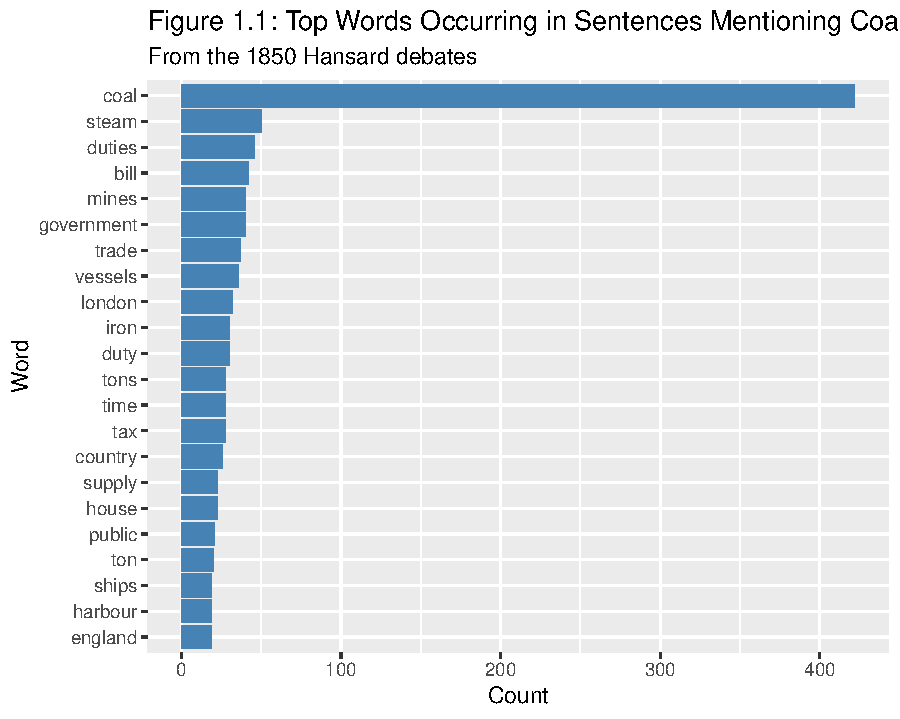
\includegraphics[width=0.8\linewidth]{ch1-11.25.2024_files/figure-latex/unnamed-chunk-29-1}

The resulting bar chart shows us the number of times ``coal'' was
mentioned, as well as the top words that appear with coal. Note that
because we are analyzing collocates, these counts do not reflect the
total number of times they were mentioned between 1850 to 1859. Instead,
the counts represent the total number of times these words appear in the
same context as ``coal.''

The second most frequent word is ``steam'' followed by ``duties,''
``bill,'' and ``mines.'' Words like ``duty,'' ``iron,'' ``tax,'' and
``supply'' indicate key economic and industrial topics related to coal
during the debates, with ``iron'' possibly tied to the role of coal in
iron production. ``Harbour,'' ``ships,'' and ``vessels'' suggest
discussions related to transportation and trade of coal.

Rather than focusing on specific speeches, this method of visualizing
data allows us to trace broader semantic and thematic structures that
shaped the discourse around the keyword coal in the 1850s. By
aggregating linguistic data over time, we can detect not only the
persistence of industrial and economic concerns, but also a macroscopic
view of historical language.

Taken together, the visualization emphasizes the central role of coal in
the British economy and legislation in the 1850s, as well as its links
to other industrial and governmental matters. The visualization also
reflects concerns around infrastructure, taxation, and policy decisions
regarding coal. Our analysis will gain nuance the more we compare near
concepts. While coal was important to powering Britain's industrial
revolution, perhaps the most controversial economic debates of the 1850s
revolved around the issue of the Corn Laws, the system of taxation of
wheat and other grains, which were originally introduced to protect
British farmers. Working-class demands for cheap bread led to the repeal
of the Corn Laws in 1846. Knowledge of these facts might lead us to ask:
were coal and corn debated using the same language or different words?

\begin{Shaded}
\begin{Highlighting}[]
\CommentTok{\# filter the dataset to include only rows where the word "corn" appears as a whole word}
\CommentTok{\# tokenize the filtered text into individual lowercase words}
\CommentTok{\# remove stop words that carry little semantic weight}
\CommentTok{\# exclude any tokens containing digits (e.g., "1850", "2nd")}
\CommentTok{\# count the frequency of each remaining word}
\CommentTok{\# sort the words in descending order of frequency}
\NormalTok{corn\_context }\OtherTok{\textless{}{-}}\NormalTok{ hansard\_1850 }\SpecialCharTok{\%\textgreater{}\%} \CommentTok{\# create a new data frame}
  \FunctionTok{filter}\NormalTok{(}\FunctionTok{str\_detect}\NormalTok{(text, }\StringTok{"}\SpecialCharTok{\textbackslash{}\textbackslash{}}\StringTok{bcorn}\SpecialCharTok{\textbackslash{}\textbackslash{}}\StringTok{b"}\NormalTok{)) }\SpecialCharTok{\%\textgreater{}\%} \CommentTok{\# filter rows with \textquotesingle{}corn\textquotesingle{} as a whole word}
  \FunctionTok{unnest\_tokens}\NormalTok{(word, text) }\SpecialCharTok{\%\textgreater{}\%} \CommentTok{\# tokenize text}
  \FunctionTok{anti\_join}\NormalTok{(stop\_words) }\SpecialCharTok{\%\textgreater{}\%} \CommentTok{\# remove stop words}
  \FunctionTok{filter}\NormalTok{(}\SpecialCharTok{!}\FunctionTok{str\_detect}\NormalTok{(word, }\StringTok{"[:digit:]"}\NormalTok{)) }\SpecialCharTok{\%\textgreater{}\%} \CommentTok{\# remove tokens with digits}
  \FunctionTok{count}\NormalTok{(word) }\SpecialCharTok{\%\textgreater{}\%} \CommentTok{\# count word frequency}
  \FunctionTok{arrange}\NormalTok{(}\FunctionTok{desc}\NormalTok{(n)) }\CommentTok{\# sort by frequency}
\end{Highlighting}
\end{Shaded}

\begin{Shaded}
\begin{Highlighting}[]
\FunctionTok{head}\NormalTok{(corn\_context)}
\end{Highlighting}
\end{Shaded}

\begin{verbatim}
##      word    n
## 1    corn 2085
## 2    laws  556
## 3 country  426
## 4    duty  333
## 5   price  325
## 6  repeal  274
\end{verbatim}

Already we can see the words that most frequently co-occurred with our
keyword ``corn.'' Visualizing the top 20 words using \texttt{ggplot}
makes this context easier to apprehend.

\begin{Shaded}
\begin{Highlighting}[]
\CommentTok{\# select the 20 most frequent words from the corn{-}related word counts}
\CommentTok{\# this subset will be used to visualize the most relevant terms}
\NormalTok{top\_corn }\OtherTok{\textless{}{-}}\NormalTok{ corn\_context }\SpecialCharTok{\%\textgreater{}\%}
  \FunctionTok{top\_n}\NormalTok{(}\DecValTok{20}\NormalTok{)  }\CommentTok{\# top 20 words}
\end{Highlighting}
\end{Shaded}

\begin{verbatim}
## Selecting by n
\end{verbatim}

\begin{Shaded}
\begin{Highlighting}[]
\CommentTok{\# create a horizontal bar plot showing word frequencies}
\CommentTok{\# this plot highlights the most common words in sentences mentioning "corn"}
\FunctionTok{ggplot}\NormalTok{(}\AttributeTok{data =}\NormalTok{ top\_corn) }\SpecialCharTok{+}
  \FunctionTok{geom\_col}\NormalTok{(}\FunctionTok{aes}\NormalTok{(}\AttributeTok{x =} \FunctionTok{reorder}\NormalTok{(word, n), }\AttributeTok{y =}\NormalTok{ n), }\CommentTok{\# draw bars sorted by count}
           \AttributeTok{fill =} \StringTok{"steel blue"}\NormalTok{) }\SpecialCharTok{+} \CommentTok{\# set bar color}
  \FunctionTok{coord\_flip}\NormalTok{() }\SpecialCharTok{+} \CommentTok{\# flip axes for horizontal bars}
  \FunctionTok{labs}\NormalTok{(}\AttributeTok{title =} \StringTok{"Top Words Occurring in Sentences Mentioning Corn"}\NormalTok{, }\CommentTok{\# add title}
       \AttributeTok{subtitle =} \StringTok{"From the 1850 Hansard debates"}\NormalTok{, }\CommentTok{\# add subtitle}
       \AttributeTok{x =} \StringTok{"Word"}\NormalTok{, }\CommentTok{\# x{-}axis label}
       \AttributeTok{y =} \StringTok{"Count"}\NormalTok{) }\CommentTok{\# y{-}axis label}
\end{Highlighting}
\end{Shaded}

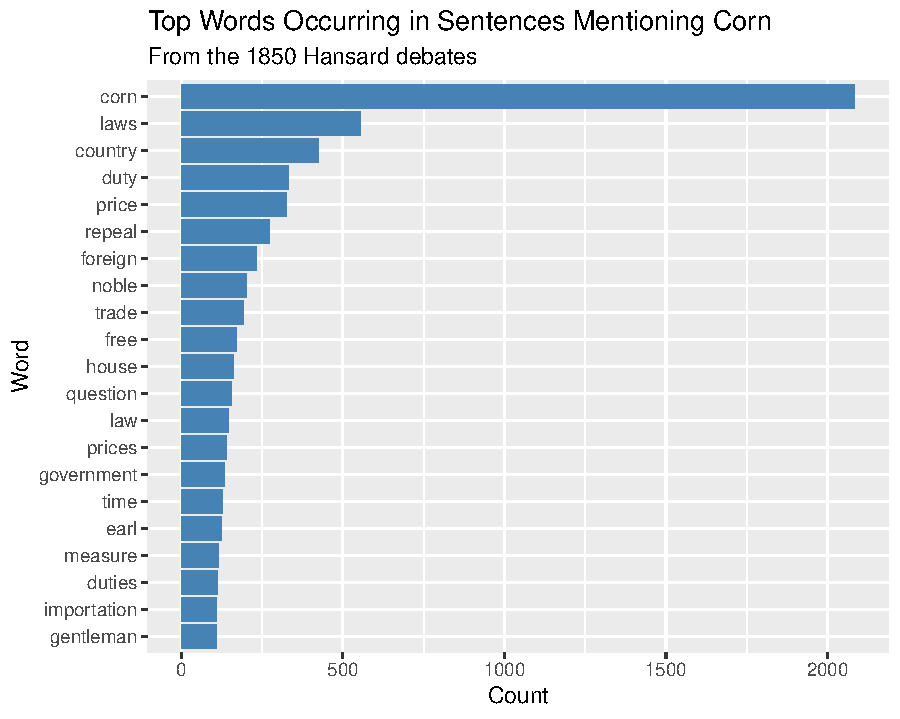
\includegraphics[width=0.8\linewidth]{ch1-11.25.2024_files/figure-latex/unnamed-chunk-32-1}

Comparison between the words used in the context of coal and corn gives
us a foothold for beginning to think about how taxation was discussed in
different contexts. For instance, the context of both keywords reference
the role of ``time'', ``duties'', ``taxes'', and the ``government'', but
debates over corn are more linked to the question of Britain's
dependence ``foreign'' powers, whereas debates over coal are more
crucially related to the condition of ``England'' itself.

Further research would be necessary for an analyst to decide whether
comparing these two commodities as keywords is worthwhile, and which
collocates offer insight. Nevertheless, at this point we have
demonstrated a preliminary process with which most of the analyses in
this book will start: by loading data, inspecting data, breaking that
data into words, and counting those words. Later chapters will
complicate this process, giving us more sophisticated approaches to
understanding historical change and change over time.

This foundational workflow, loading, inspecting, tokenizing, and
counting words, lays the groundwork for more nuanced textual inquiries.
One such method, which begins to address the limitations of mere
frequency counts, is the ``Keywords in Context'' (KWIC) approach.

\subsection{Finding a Word's Context using ``Keywords in Context''
(KWIC)}\label{finding-a-words-context-using-keywords-in-context-kwic}

In the 1950s, Jesuit scholar Father Roberto Busa partnered with IBM to
create a machine-readable concordance of the works of Thomas Aquinas,
known as the Corpus Thomisticum (Jones 2016). As a Jesuit scholar deeply
immersed in Thomistic philosophy, Busa wanted to analyze the use and
meaning of the Latin word ``in''---a preposition with significant
theological weight---in the complete works of Thomas Aquinas. These
texts contained over 11 million words, making it virtually impossible to
conduct such a study without first restructuring the material for
analysis. However, the challenge he faced was not only the scale of the
corpus, but the need to preserve the linguistic and philosophical nuance
of Aquinas's writings.

Widely regarded as the inception of the digital humanities, Busa's work
demonstrated the transformational potential of computing for humanistic
inquiry. Busa's project marked a pivotal shift in textual scholarship by
introducing computational methods to the humanities. By producing a
machine-readable concordance of Thomas Aquinas's works, the project laid
the foundation for techniques now central to digital textual analysis,
including the use of KWIC (Keywords in Context) displays.

Concordance-style views have remained central to the study of language
and meaning in the humanities. While collocates are one way to explore a
word's context---by analyzing frequently co-occurring tokens---they are
not the only method. Tools like ``Keywords in Context'' (KWIC),
available in the \texttt{quanteda} library, provide a concordance-style
view that presents sentence-level context. This allows researchers to
examine not just which words appear near each other, but how a term
functions within its surrounding textual context

To look at just the month of February, we need to load our decade subset
that contains information about dates, called
\texttt{debate\_metadata\_1850}, and join it with the dataset containing
the debates, \texttt{hansard\_1850}.

\begin{Shaded}
\begin{Highlighting}[]
\CommentTok{\# Load the debate metadata for 1850}
\FunctionTok{data}\NormalTok{(}\StringTok{"debate\_metadata\_1850"}\NormalTok{)}
\end{Highlighting}
\end{Shaded}

\begin{Shaded}
\begin{Highlighting}[]
\FunctionTok{head}\NormalTok{(debate\_metadata\_1850)}
\end{Highlighting}
\end{Shaded}

\begin{verbatim}
##   sentence_id speechdate                       debate
## 1 S3V0108P0_0 1850-01-31       MEETING OF PARLIAMENT.
## 2 S3V0108P0_1 1850-01-31       MEETING OF PARLIAMENT.
## 3 S3V0108P0_2 1850-01-31 SCOTCH REPRESENTATIVE PEERS.
## 4 S3V0108P0_3 1850-01-31 SCOTCH REPRESENTATIVE PEERS.
## 5 S3V0108P0_4 1850-01-31 SCOTCH REPRESENTATIVE PEERS.
## 6 S3V0108P0_5 1850-01-31 SCOTCH REPRESENTATIVE PEERS.
\end{verbatim}

We will cover joins in greater detail in Chapter 2. For now it's just
important to know that we are using our unique ID,
\texttt{sentence\_id}, to join the two data frames together so that the
speeches are aligned with their correct dates.

\begin{Shaded}
\begin{Highlighting}[]
\CommentTok{\# Merge the hansard\_1850 text data with its corresponding metadata}
\CommentTok{\# using a left join to keep all rows from hansard\_1850}
\NormalTok{hansard\_1850\_with\_metadata }\OtherTok{\textless{}{-}} \FunctionTok{left\_join}\NormalTok{(hansard\_1850, debate\_metadata\_1850)}
\end{Highlighting}
\end{Shaded}

\begin{Shaded}
\begin{Highlighting}[]
\FunctionTok{head}\NormalTok{(hansard\_1850\_with\_metadata)}
\end{Highlighting}
\end{Shaded}

\begin{verbatim}
##   sentence_id
## 1 S3V0108P0_0
## 2 S3V0108P0_1
## 3 S3V0108P0_2
## 4 S3V0108P0_3
## 5 S3V0108P0_4
## 6 S3V0108P0_5
##                                                                                                                                                                                                                                                                                                                                                                                                                                                          text
## 1                                                                                                                                                                                                                       , which had been prorogued successively from the 1st of August to the 9th of October, from thence to the 20th of November, thence to the 16th of January, and from thence to the 31st January, met this day for despatch of business.
## 2                                                                                                                                             The Parliament was opened by Commission, the LORDS COMMISSIONERS present being the LORD CHANCELLOR; the LORD PRESIDENT OF THE COUNCIL (the Marquess of Lansdowne); the LORD PRIVY SEAL (the Earl of Minto); the LORD CHAMBERLAIN OF THE HOUSEHOLD (the Marquess of Breadalbane); and the LORD BISHOP OF LONDON.
## 3                                                                                                                                                                                                                                                                                 called attention to a great omission of their duty on the part of Ministers, with respect to the privileges of their Lordships, which might and ought to have been avoided.
## 4                                                                                                                                                                                                                                                                                                      At pre-sent there were two vacancies in the representative Peers of Scotland, in consequence of the deaths of the Earl of Airlie and of Lord Colville.
## 5 Although the Act of Parliament directed that the proclamation should issue forthwith for the election of representative Peers to fill up any vacancies which might occur, by death or otherwise, no such proclamation had yet taken place in the case of the two vacancies he had just mentioned, and the consequence was, that for twenty-four days after the meeting of Parliament it was not possible for any Scotch representative Peers to be elected.
## 6                                                                                                                                                                                                                                                                                                                                                           The Peerage of Scotland was not therefore represented in Parliament at present as it ought to be.
##   speechdate                       debate
## 1 1850-01-31       MEETING OF PARLIAMENT.
## 2 1850-01-31       MEETING OF PARLIAMENT.
## 3 1850-01-31 SCOTCH REPRESENTATIVE PEERS.
## 4 1850-01-31 SCOTCH REPRESENTATIVE PEERS.
## 5 1850-01-31 SCOTCH REPRESENTATIVE PEERS.
## 6 1850-01-31 SCOTCH REPRESENTATIVE PEERS.
\end{verbatim}

In the following code we filter for speech dates that are on or after
(greater than or equal to \texttt{\textgreater{}=}) February 1, 1850,
and on or before (less than or equal to \texttt{\textless{}=}) February
28, 1850.

\begin{Shaded}
\begin{Highlighting}[]
\CommentTok{\# Filter the dataset to include only speeches from February 1850}
\NormalTok{top\_month }\OtherTok{\textless{}{-}}\NormalTok{ hansard\_1850\_with\_metadata }\SpecialCharTok{\%\textgreater{}\%} \CommentTok{\# create a new data frame}
  \FunctionTok{filter}\NormalTok{(speechdate }\SpecialCharTok{\textgreater{}=} \StringTok{"1850{-}02{-}01"}\NormalTok{, }\CommentTok{\# filter}
\NormalTok{         speechdate }\SpecialCharTok{\textless{}=} \StringTok{"1850{-}02{-}28"}\NormalTok{)}
\end{Highlighting}
\end{Shaded}

KWIC returns a concordance-style text output with the words that come
directly before and after the keyword in a sentence. Quanteda's version
of \texttt{KWIC()} uses a different approach from \texttt{tidyverse}. It
processes data quicker if we first transform the data from a tidy table
into a ``quanteda corpus'' using \texttt{corpus()}. Using this approach,
we can tell Quanteda that we wish to process the \texttt{text} column.

When using \texttt{KWIC()} we can specify the keyword, the maximum
number of words to display before and after the keyword, and we can also
tell \texttt{KWIC()} to do a case insensitive match so that we match
with uppercase or lowercase instances of our keyword.

\begin{Shaded}
\begin{Highlighting}[]
\CommentTok{\# load the quanteda package}
\FunctionTok{library}\NormalTok{(quanteda)}
\end{Highlighting}
\end{Shaded}

\begin{verbatim}
## Package version: 4.3.1
## Unicode version: 14.0
## ICU version: 70.1
\end{verbatim}

\begin{verbatim}
## Parallel computing: disabled
\end{verbatim}

\begin{verbatim}
## See https://quanteda.io for tutorials and examples.
\end{verbatim}

\begin{Shaded}
\begin{Highlighting}[]
\CommentTok{\# convert the filtered february 1850 dataset into a quanteda corpus object}
\CommentTok{\# specify that the \textquotesingle{}text\textquotesingle{} column contains the actual speech content}
\NormalTok{my\_corpus }\OtherTok{\textless{}{-}} \FunctionTok{corpus}\NormalTok{(top\_month, }\AttributeTok{text\_field =} \StringTok{"text"}\NormalTok{) }

\CommentTok{\# search for instances of the word "corn" in the corpus}
\CommentTok{\# extract 5 words before and after each occurrence}
\CommentTok{\# make the search case{-}insensitive so it matches "corn", "Corn", etc.}
\NormalTok{corn\_kwic }\OtherTok{\textless{}{-}} \FunctionTok{kwic}\NormalTok{(}\FunctionTok{tokens}\NormalTok{(my\_corpus), }\CommentTok{\# tokenize corpus}
                  \StringTok{"corn"}\NormalTok{, }\CommentTok{\# keyword to search}
                  \AttributeTok{window =} \DecValTok{5}\NormalTok{, }\CommentTok{\# number of words before/after}
                  \AttributeTok{case\_insensitive =} \ConstantTok{TRUE}\NormalTok{) }\CommentTok{\# match regardless of case}
\end{Highlighting}
\end{Shaded}

\begin{Shaded}
\begin{Highlighting}[]
\FunctionTok{head}\NormalTok{(corn\_kwic)}
\end{Highlighting}
\end{Shaded}

\begin{verbatim}
## Keyword-in-context with 6 matches.                                                            
##   [text2032, 7]             cultivation of land, as | corn |
##  [text2036, 11]           south of Ireland dealt in | corn |
##  [text2038, 13] , deterred persons from cultivating | corn |
##   [text2536, 2]                                  on | corn |
##  [text2568, 23]         laws governing the price of | corn |
##  [text2578, 13]                to the repeal of the | corn |
##                         
##  ground, being given up 
##  , and were the pro     
##  .                      
##  , would never have been
##  .                      
##  laws, for those laws
\end{verbatim}

\subsection{Critical Thinking With
Collocates}\label{critical-thinking-with-collocates}

When is collocate analysis the right method? Researchers of conceptual
history frequently use collocates to understand the subtle differences
between synonyms. For instance, historian Ruben Ros (2021) has
investigated the way that Dutch newspapers in the nineteenth century
began to use terms such as ``foreign,'' ``overseas,'' and ``strange'' in
the process of constructing a narrative that increasingly linked the
dangers of foreign influence and suspicion of ethnic minorities.

With collocate analysis alone, we cannot trace discourses over time -- a
crucial step in understanding the construction of political and cultural
positions. But we can begin to tease apart the meanings of
closely-related ideas at various points in the past. We can recreate
Ro's approach in miniature here, asking the question: how did British
members of parliament in the 1850s talk about foreigners and colonial
subjects?

In the following code we create a function for filtering the Hansard
data for a keyword, and visualizing the top 20 words. These are the same
series of steps we have performed already, but here we are using our
function to produce a series of related graphs in succession without
writing out the same instructions multiple times.

Creating a function will allow us to automatically create a series of
graphs for the keywords we wish to analyze. Producing many graphs in
succession is good practice for exploratory data analysis (EDA), the
stage of research where we look at the data to understand its basic
patterns, structure, and possible meanings before doing formal
interpretation or modeling. Performing a comparative analysis of graphs
side-by-side is one of the main skills digital humanists use when
considering the subtle structures of meaning and difference that define
cultural and political conversations. A careful comparison between the
charts above offers the beginnings of a nuanced analysis of overlapping
terms used by British members of parliament to refer to people and
forces from beyond Britain.

\begin{Shaded}
\begin{Highlighting}[]
\CommentTok{\# define a function to generate a bar plot of top words that co{-}occur with a given keyword}
\CommentTok{\# filters the dataset for rows containing the keyword as a whole word}
\CommentTok{\# tokenizes the text, removes stop words and numeric tokens}
\CommentTok{\# keeps the top 20 most frequent words and plots them as a horizontal bar chart}
\NormalTok{generate\_word\_plot }\OtherTok{\textless{}{-}} \ControlFlowTok{function}\NormalTok{(keyword, hansard\_data) \{}
    
\NormalTok{    filtered\_hansard\_1850 }\OtherTok{\textless{}{-}}\NormalTok{ hansard\_data }\SpecialCharTok{\%\textgreater{}\%}
      \FunctionTok{filter}\NormalTok{(}\FunctionTok{str\_detect}\NormalTok{(text, }\FunctionTok{paste0}\NormalTok{(}\StringTok{"}\SpecialCharTok{\textbackslash{}\textbackslash{}}\StringTok{b"}\NormalTok{, keyword, }\StringTok{"}\SpecialCharTok{\textbackslash{}\textbackslash{}}\StringTok{b"}\NormalTok{))) }\SpecialCharTok{\%\textgreater{}\%} \CommentTok{\# filter rows with keyword}
      \FunctionTok{unnest\_tokens}\NormalTok{(word, text) }\SpecialCharTok{\%\textgreater{}\%} \CommentTok{\# tokenize text}
      \FunctionTok{anti\_join}\NormalTok{(stop\_words) }\SpecialCharTok{\%\textgreater{}\%} \CommentTok{\# remove stop words}
      \FunctionTok{filter}\NormalTok{(}\SpecialCharTok{!}\FunctionTok{str\_detect}\NormalTok{(word, }\StringTok{"[:digit:]"}\NormalTok{)) }\SpecialCharTok{\%\textgreater{}\%} \CommentTok{\# remove numeric tokens}
      \FunctionTok{count}\NormalTok{(word) }\SpecialCharTok{\%\textgreater{}\%} \CommentTok{\# count word frequency}
      \FunctionTok{top\_n}\NormalTok{(}\DecValTok{20}\NormalTok{) }\CommentTok{\# keep top 20 words}
    
\NormalTok{    plot }\OtherTok{\textless{}{-}} \FunctionTok{ggplot}\NormalTok{(filtered\_hansard\_1850) }\SpecialCharTok{+} \CommentTok{\# create a new dataset for the plot                       }
      \FunctionTok{geom\_col}\NormalTok{(}\FunctionTok{aes}\NormalTok{(}\AttributeTok{x =} \FunctionTok{reorder}\NormalTok{(word, n), }\AttributeTok{y =}\NormalTok{ n), }\CommentTok{\# bar chart ordered by count}
               \AttributeTok{fill =} \StringTok{"steel blue"}\NormalTok{) }\SpecialCharTok{+} \CommentTok{\# set bar color}
      \FunctionTok{coord\_flip}\NormalTok{() }\SpecialCharTok{+} \CommentTok{\# horizontal bars}
      \FunctionTok{labs}\NormalTok{(}\AttributeTok{title =} \FunctionTok{paste}\NormalTok{(}\StringTok{"Top Words Occurring in Sentences Mentioning"}\NormalTok{, }
                         \FunctionTok{toupper}\NormalTok{(keyword)), }\CommentTok{\# plot title}
           \AttributeTok{subtitle =} \StringTok{"From the 1850 Hansard debates"}\NormalTok{, }\CommentTok{\# plot subtitle}
           \AttributeTok{x =} \StringTok{"Word"}\NormalTok{, }\CommentTok{\# x{-}axis label}
           \AttributeTok{y =} \StringTok{"Count"}\NormalTok{) }\CommentTok{\# y{-}axis label}
    
    \FunctionTok{print}\NormalTok{(plot) \} }\CommentTok{\# display the plot}
\end{Highlighting}
\end{Shaded}

\begin{Shaded}
\begin{Highlighting}[]
\CommentTok{\# use our function to create a clean bar plot of the top 20 words in sentences }
\CommentTok{\# mentioning the word "foreign"}
\FunctionTok{generate\_word\_plot}\NormalTok{(}\StringTok{"foreign"}\NormalTok{, hansard\_1850)}
\end{Highlighting}
\end{Shaded}

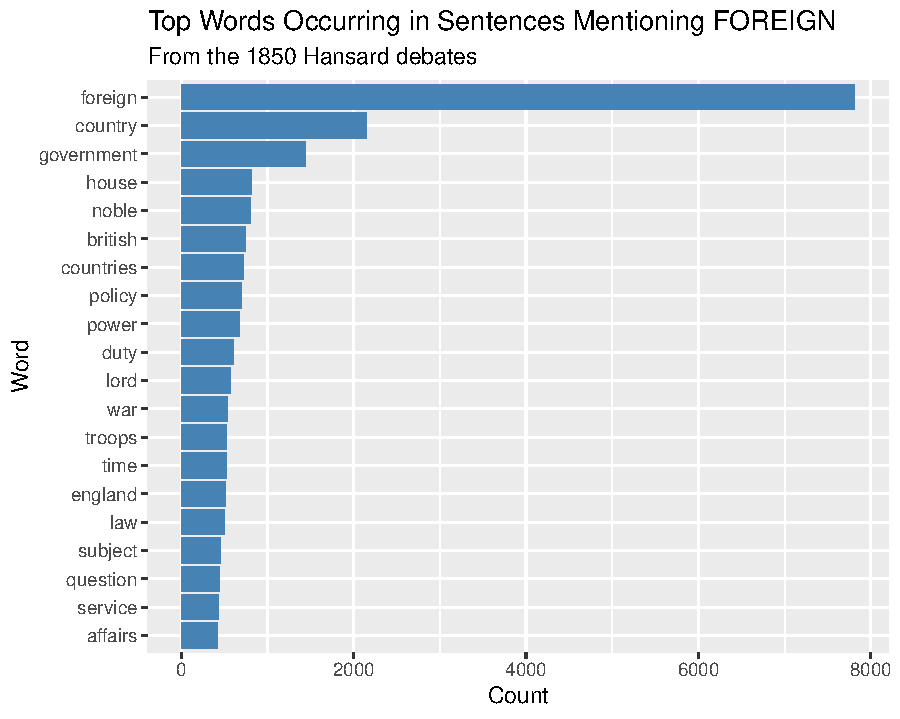
\includegraphics[width=0.8\linewidth]{ch1-11.25.2024_files/figure-latex/unnamed-chunk-41-1}

\begin{Shaded}
\begin{Highlighting}[]
\CommentTok{\# do the same for sentences that mention the word "colonial"}
\FunctionTok{generate\_word\_plot}\NormalTok{(}\StringTok{"colonial"}\NormalTok{, hansard\_1850)}
\end{Highlighting}
\end{Shaded}

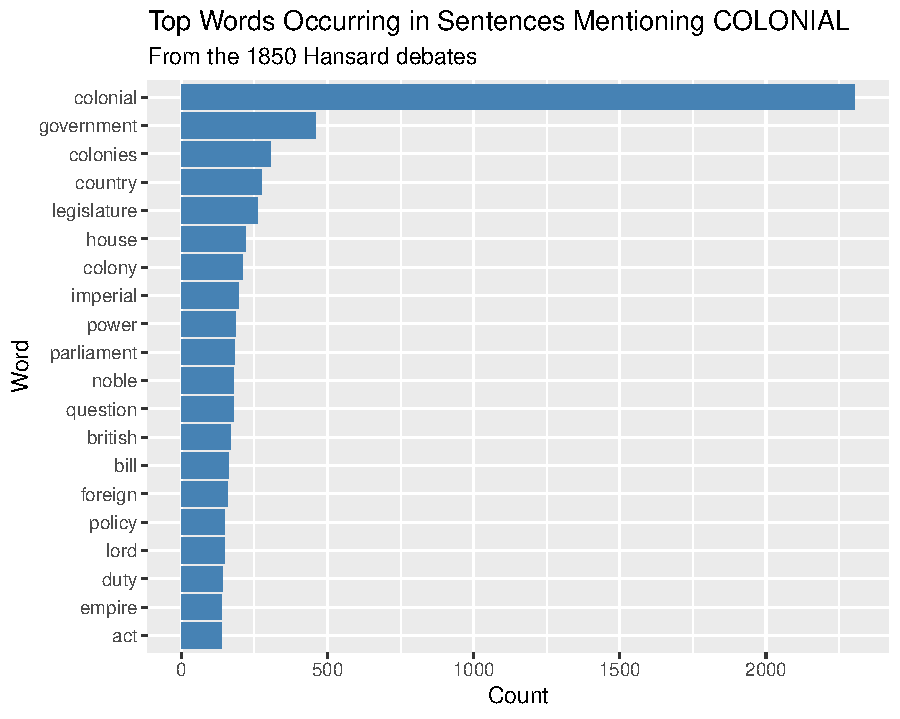
\includegraphics[width=0.8\linewidth]{ch1-11.25.2024_files/figure-latex/unnamed-chunk-42-1}

\begin{Shaded}
\begin{Highlighting}[]
\CommentTok{\# do the same for sentences that mention the word "savage"}
\FunctionTok{generate\_word\_plot}\NormalTok{(}\StringTok{"savage"}\NormalTok{, hansard\_1850)}
\end{Highlighting}
\end{Shaded}

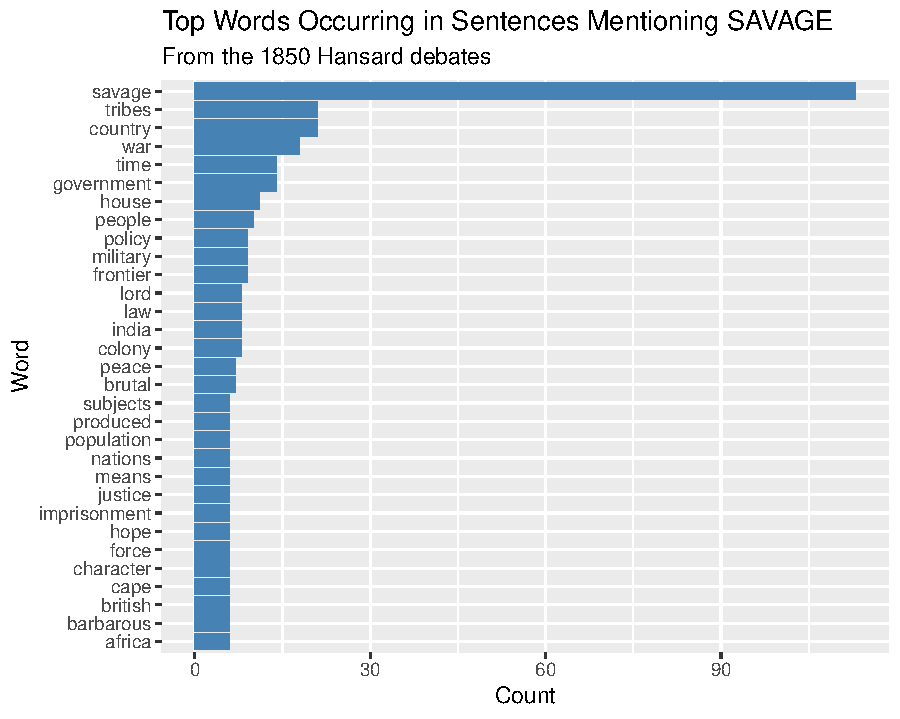
\includegraphics[width=0.8\linewidth]{ch1-11.25.2024_files/figure-latex/unnamed-chunk-43-1}

\begin{Shaded}
\begin{Highlighting}[]
\CommentTok{\# do the same for sentences that mention the word "native"}
\FunctionTok{generate\_word\_plot}\NormalTok{(}\StringTok{"native"}\NormalTok{, hansard\_1850)}
\end{Highlighting}
\end{Shaded}

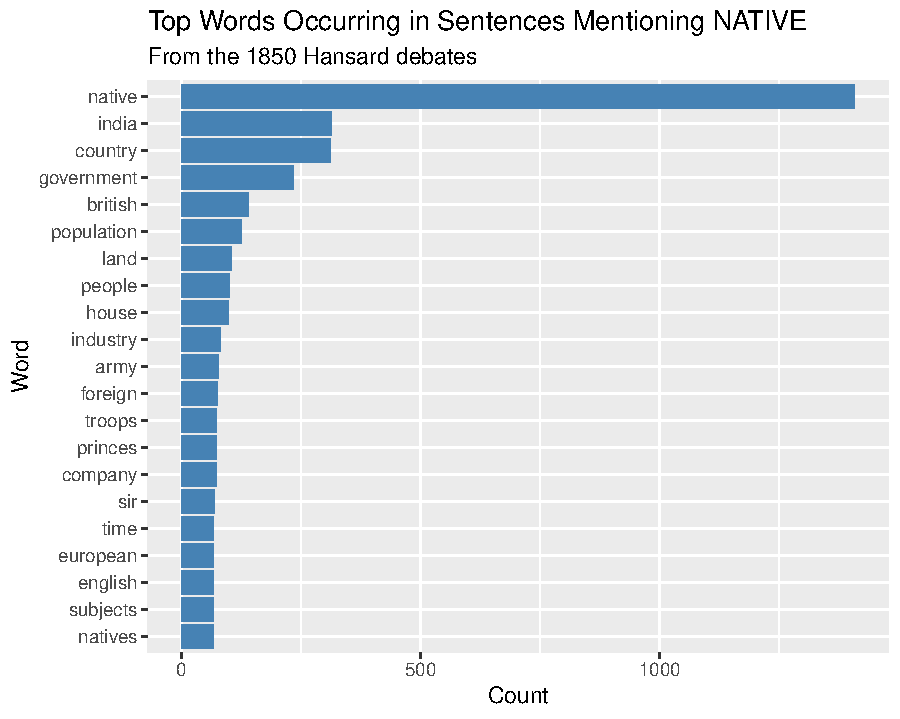
\includegraphics[width=0.8\linewidth]{ch1-11.25.2024_files/figure-latex/unnamed-chunk-44-1}

\begin{Shaded}
\begin{Highlighting}[]
\CommentTok{\# do the same for sentences that mention the word "barbarian"}
\FunctionTok{generate\_word\_plot}\NormalTok{(}\StringTok{"barbarian"}\NormalTok{, hansard\_1850)}
\end{Highlighting}
\end{Shaded}

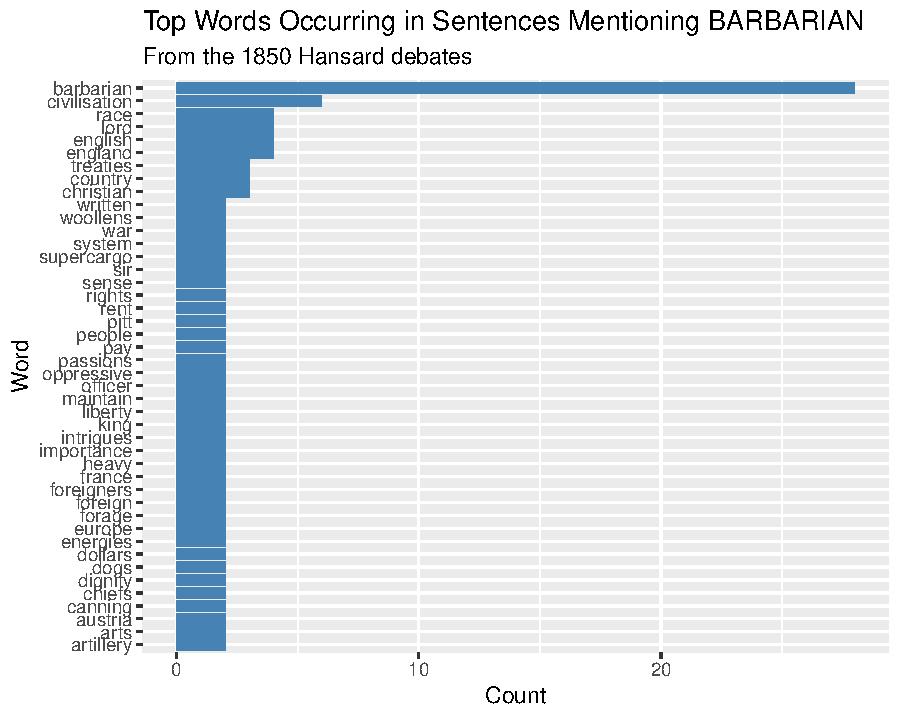
\includegraphics[width=0.8\linewidth]{ch1-11.25.2024_files/figure-latex/unnamed-chunk-45-1}

Producing many graphs in succession can be useful for exploratory data
analysis. Performing a comparative analysis of graphs side-by-side is
one of the main skills digital humanists use when considering the subtle
structures of meaning and difference that define cultural and political
conversations. A careful comparison between the charts above offers the
beginnings of a nuanced analysis of overlapping terms used by British
members of parliament to refer to people and forces from beyond Britain.

In the results, we see several closely related terms which compose a
field of interrelated meanings. Together, these terms sketch out the
diversity of contrasting ways that British members of parliament spoke
about the world outside of Britain. Some of the attributes ascribed to
the foreign were neutral in value -- for instance, the ``foreign'' was
mainly spoken about in terms of ``laws'', ``duties'', ``trade'', and
``protection'', a world in which different nations ``competed,'' but
generally not a space of moral inferiority and superiority. By contrast,
terms such as ``savage'' and ``barbarian'' telegraphed intellectual and
ethical judgments (for instance, ``brutal'') onto cultures outside of
Britain, typically associating inferiority with racial identity (Metcalf
1995, Colley 1992, Said 1987).

With these terms, a set of binaries is set up by the speakers of
Parliament, dividing the world into ``barbarian'' cultures and
``christian'' ``civilisations,'' a distinction that may have been
analyzed in terms of ``rights,'' ``treaties,'' ``war,'' ``rents,''
``passions,'' ``liberty,'' and ``energies. The distinctions between
the''foreign'' and the ``barbarian'' are invoked in relationship to the
same abstractions we saw typifying the ``foreign,'' including ``law,''
the ``country,'' and ``treaties.'' We also see the ``barbarian'' being
invoked in discussions of many commodities, including ``woolens,''
``forage,'' and ``rent.'' Indeed, the frequent invocation of law,
rights, and foreignness alongside discussions of the barbarian and the
savage suggests that the judgments ascribed to race actually bled into
conversations about law, tariffs, trade, and protectionism, perhaps as
justification for invoking British superiority.

Some readers may assume that we are performing contemporary prejudices
about racism, but the point of this exercise is that it is grounded in a
detailed and careful examination of the words counted by computational
methods. The paragraph above is not concocted out of thin air; it is an
objective description of the prejudices on display in a quantitative
reading of how British members of parliament spoke about the world
beyond their nation. We emphasize that this analysis of the related
language of the ``foreign'' and the ``barbarian'' is not concocted on
the basis of our readings of contemporary theories about racism, but is
actually derived from a careful reading of the language of Hansard, as
well as immersion in writing about the history of empire.

In general, descriptions of arguments made on the basis of word counts
tend to be more persuasive when they take on every word in a list.
Critical thinking about the meaning of proximate keywords is enhanced
when the analyst slows down, taking the trouble to examine the
distinctiveness of each individual keyword and its context. In a further
analysis, the scholar might ask questions that require examining the
results in more detail. They might ask: What biases does each term
convey? Where do the terms overlap? What new information is encapsulated
by some words but not others? We could continue this line of inquiry to
trace the keyword-context pairs back to their original context in
sentences and speeches on the page, showing how speakers used these
words to formulate actual arguments with consequences for the
development of nations and their economies.

Examining collocates provides the basis for critical thinking about the
changing and overlapping meaning of shared concepts in the human past.
Skillful analysts can use approaches of this kind to examine the meaning
of language about categories beyond those of gender, race, nationality,
and commodities, asking questions about the intellectual categories that
governed how members of parliament understood governance itself,
economics, truth, science, virtue, economics, and reason itself. In
every case, the approach would be the same: to examine not merely one or
two keywords, but many related keywords, drawing attention to the subtle
overlap and differences between the terms in usage, and how those
overlapping concepts together work to produce a field of meaning.

\subsection{Critical Thinking About Data and its
Limits}\label{critical-thinking-about-data-and-its-limits}

Another fruitful avenue for critical thinking is the question of which
problems are suited to textual analysis and which are not. Skillful
analysts are wary of asking the wrong question with the wrong tool.
Among the techniques that we have learned in this chapter is the ability
to load and inspect data. Inspecting the data allows the analyst to
notice issues caused by computational processing of text that may cause
issues down the line unless the analyst is aware of them.

Looking at the first lines of \texttt{hansard\_1850}, you might ask
yourself these questions: are all of the lines in the ``text'' field
actually sentences? Are all the words in the same style with respect to
capitalization? We can inspect this further.

Analyzing the entire data frame to further inspect the data can be
distracting since a data frame usually contains multiple columns, some
which may be irrelevant to our current query.

\begin{Shaded}
\begin{Highlighting}[]
\FunctionTok{head}\NormalTok{(hansard\_1850\_with\_metadata)}
\end{Highlighting}
\end{Shaded}

\begin{verbatim}
##   sentence_id
## 1 S3V0108P0_0
## 2 S3V0108P0_1
## 3 S3V0108P0_2
## 4 S3V0108P0_3
## 5 S3V0108P0_4
## 6 S3V0108P0_5
##                                                                                                                                                                                                                                                                                                                                                                                                                                                          text
## 1                                                                                                                                                                                                                       , which had been prorogued successively from the 1st of August to the 9th of October, from thence to the 20th of November, thence to the 16th of January, and from thence to the 31st January, met this day for despatch of business.
## 2                                                                                                                                             The Parliament was opened by Commission, the LORDS COMMISSIONERS present being the LORD CHANCELLOR; the LORD PRESIDENT OF THE COUNCIL (the Marquess of Lansdowne); the LORD PRIVY SEAL (the Earl of Minto); the LORD CHAMBERLAIN OF THE HOUSEHOLD (the Marquess of Breadalbane); and the LORD BISHOP OF LONDON.
## 3                                                                                                                                                                                                                                                                                 called attention to a great omission of their duty on the part of Ministers, with respect to the privileges of their Lordships, which might and ought to have been avoided.
## 4                                                                                                                                                                                                                                                                                                      At pre-sent there were two vacancies in the representative Peers of Scotland, in consequence of the deaths of the Earl of Airlie and of Lord Colville.
## 5 Although the Act of Parliament directed that the proclamation should issue forthwith for the election of representative Peers to fill up any vacancies which might occur, by death or otherwise, no such proclamation had yet taken place in the case of the two vacancies he had just mentioned, and the consequence was, that for twenty-four days after the meeting of Parliament it was not possible for any Scotch representative Peers to be elected.
## 6                                                                                                                                                                                                                                                                                                                                                           The Peerage of Scotland was not therefore represented in Parliament at present as it ought to be.
##   speechdate                       debate
## 1 1850-01-31       MEETING OF PARLIAMENT.
## 2 1850-01-31       MEETING OF PARLIAMENT.
## 3 1850-01-31 SCOTCH REPRESENTATIVE PEERS.
## 4 1850-01-31 SCOTCH REPRESENTATIVE PEERS.
## 5 1850-01-31 SCOTCH REPRESENTATIVE PEERS.
## 6 1850-01-31 SCOTCH REPRESENTATIVE PEERS.
\end{verbatim}

We can make the data more readable by displaying just the data from the
column of interest.

In the following code, we use \texttt{hansard\_1850{[}1:10,\ 2{]}} to
select a specific item from \texttt{hansard\_1850}.
\texttt{hansard\_1850} refers to a data frame or matrix, and
\texttt{{[}1,\ 2{]}} refers to the row and column indices we wish to
look at. The structure of the syntax is this:
\texttt{{[}row,\ column{]}}. The numeric range, \texttt{1:10}, in the
``row'' field tells R to display rows 1 to 10. We put ``2'' in the
``column'' field to tell R to display just the second column, which in
this case is the column containing text.

\begin{Shaded}
\begin{Highlighting}[]
\CommentTok{\# view rows 1 to 10 from the 2nd column of the hansard\_1850 dataset}
\NormalTok{hansard\_1850[}\DecValTok{1}\SpecialCharTok{:}\DecValTok{10}\NormalTok{, }\DecValTok{2}\NormalTok{]}
\end{Highlighting}
\end{Shaded}

\begin{longtable}[]{@{}
  >{\raggedright\arraybackslash}p{(\linewidth - 0\tabcolsep) * \real{1.0000}}@{}}
\toprule\noalign{}
\begin{minipage}[b]{\linewidth}\raggedright
x
\end{minipage} \\
\midrule\noalign{}
\endhead
\bottomrule\noalign{}
\endlastfoot
, which had been prorogued successively from the 1st of August to the
9th of October, from thence to the 20th of November, thence to the 16th
of January, and from thence to the 31st January, met this day for
despatch of business. \\
The Parliament was opened by Commission, the LORDS COMMISSIONERS present
being the LORD CHANCELLOR; the LORD PRESIDENT OF THE COUNCIL (the
Marquess of Lansdowne); the LORD PRIVY SEAL (the Earl of Minto); the
LORD CHAMBERLAIN OF THE HOUSEHOLD (the Marquess of Breadalbane); and the
LORD BISHOP OF LONDON. \\
called attention to a great omission of their duty on the part of
Ministers, with respect to the privileges of their Lordships, which
might and ought to have been avoided. \\
At pre-sent there were two vacancies in the representative Peers of
Scotland, in consequence of the deaths of the Earl of Airlie and of Lord
Colville. \\
Although the Act of Parliament directed that the proclamation should
issue forthwith for the election of representative Peers to fill up any
vacancies which might occur, by death or otherwise, no such proclamation
had yet taken place in the case of the two vacancies he had just
mentioned, and the consequence was, that for twenty-four days after the
meeting of Parliament it was not possible for any Scotch representative
Peers to be elected. \\
The Peerage of Scotland was not therefore represented in Parliament at
present as it ought to be. \\
He wanted to know what his noble Friend the President of the Council had
to urge in defence of this omission; for certain it was that the Act of
Parliament had not been obeyed? \\
said, that the Government were not to blame for the omission, as they
had not received any requisition from the usual quarter; they had
strictly followed the previous usage. \\
said, the explanation of the noble Marquess was unsatisfactory. \\
The clause in 5 \& 6 Anne, c.~8, directed what should be done in the
case of vacancies by death, and the words could not well be
misunderstood. \\
\end{longtable}

Some of the rows in the ``text'' field appear not to be complete
sentences. We can investigate this oddity further.

\begin{Shaded}
\begin{Highlighting}[]
\CommentTok{\# view the first row from the 2nd column of the hansard\_1850 dataset}
\NormalTok{hansard\_1850[}\DecValTok{1}\NormalTok{, }\DecValTok{2}\NormalTok{]}
\end{Highlighting}
\end{Shaded}

\begin{longtable}[]{@{}
  >{\raggedright\arraybackslash}p{(\linewidth - 0\tabcolsep) * \real{1.0000}}@{}}
\toprule\noalign{}
\begin{minipage}[b]{\linewidth}\raggedright
x
\end{minipage} \\
\midrule\noalign{}
\endhead
\bottomrule\noalign{}
\endlastfoot
, which had been prorogued successively from the 1st of August to the
9th of October, from thence to the 20th of November, thence to the 16th
of January, and from thence to the 31st January, met this day for
despatch of business. \\
\end{longtable}

At this point the dataset is too broad to clearly display by printing,
and some data is cut off. To view the whole text, double-click on the
cell, copy and paste the text into a word processor. The content reads
like so:

\begin{quote}
``, which had been prorogued successively from the 1st of August to the
9th of October, from thence to the 20th of November, thence to the 16th
of January, and from thence to the 31st January, met this day for
despatch {[}sic{]} of business.''
\end{quote}

The first row appears to be a description of the opening of parliament.
Technically, it is a commentary by the printer, not a line of debate.
The convention of discussing parliament's timetables was in place in
1850, but we do not know if the printer always printed this line through
the entire century. We should be aware of this convention and curious
about it if we find ourselves counting months or discussions of words
such as ``business.''

Let's keep inspecting the data, this time turning to the third row in
our dataset.

\begin{Shaded}
\begin{Highlighting}[]
\CommentTok{\# view the third row from the 2nd column of the hansard\_1850 dataset}
\NormalTok{hansard\_1850[}\DecValTok{3}\NormalTok{, }\DecValTok{2}\NormalTok{]}
\end{Highlighting}
\end{Shaded}

\begin{longtable}[]{@{}
  >{\raggedright\arraybackslash}p{(\linewidth - 0\tabcolsep) * \real{1.0000}}@{}}
\toprule\noalign{}
\begin{minipage}[b]{\linewidth}\raggedright
x
\end{minipage} \\
\midrule\noalign{}
\endhead
\bottomrule\noalign{}
\endlastfoot
called attention to a great omission of their duty on the part of
Ministers, with respect to the privileges of their Lordships, which
might and ought to have been avoided. \\
\end{longtable}

Here, we see another sentence fragment:

\begin{quote}
``called attention to a great omission of their duty on the part of
Ministers, with respect to the privileges of their Lordships, which
might and ought to have been avoided.''
\end{quote}

The sentence fragment has resulted from attempting to process data while
working on another convention of printing: the fact that the publisher
of Hansard for much of the century gave the name of the speaker followed
by a description of the airing of the speech. On the page, we would be
given the name of a speaker or their title, for example, ``The Lord
Chancellor'' or ``Mr.~Gladstone.'' The passage of text would therefore
read, {[}the speaker{]} ``called attention to a great omission\ldots{}''
-- in other words, it would not be a sentence fragment, so much as a
journalistic description of a speaker. The actual speech probably began
with a statement something like this: ``It is a great omission of their
duty on the part of Ministers{[}\ldots{]}.'' In other words, we are
looking at an oddity that resulted from a mismatch between the
19th-century printed record and how the computer processed the data. We
compiled the data and separate all of the speaker names into one
``field'' of data, which we stored in a separate dataset, to be accessed
in Chapter 2. We have sorted all of the text into the ``text'' field,
which is held in \texttt{hansard\_1850}. The computer did not process
the journalistic description of a speech rather than a normal speech.

Looking at the data presents an opportunity for critical thinking.
Analysts of text as data routinely need to inspect their data and make
sure that the data's quality and density are sufficient to support
claims that they might make.

Already, we can see that the data has certain features that might
interfere with certain kinds of queries, and we should already be
thinking about what these limits might be. Yet the convention of
journalistic reporting on speeches can cause trouble for the analyst if
the analysts are not aware of what has changed. The conventions of
describing speeches changed over the course of the century; at the
beginning of the century, journalistic descriptions were more common.
Later in the century, the conventions changed, and many more speeches
were reported near verbatim without journalistic commentary. We should
be aware of conventions of this kind if we count words which may be
related to journalistic observations such as ``attention,'' ``spoke,''
``declared,'' and so on. Otherwise we may be tempted to interpret
changes to the publisher's conventions of printing speeches as evidence
for changing ideas about politics.

Whether or not data quality will interfere with our ability to make
inferences from the data depends on what we are asking. If we are
counting mentions of the word ``duty'' or the rest of the words in the
content of the speech, then our counts of the words will be correct. If
we contrive to study the history of journalistic observation by tracking
sentence fragments in the dataset, this data will support such a
reading. But we should be wary making inferences about any kind of
inquiry where there is a risk of overlap between substantive discussions
and journalistic observation.

\subsection{Exercises}\label{exercises}

Expand your grasp of the code and your powers of critical reflection by
trying the following exercises:

\begin{enumerate}
\def\labelenumi{\arabic{enumi})}
\item
  Alter the code above to compare the context for the keywords ``girl''
  and ``woman.'' Do you expect the context to be similar for both? Does
  anything surprise you about the results?
\item
  Use your powers of inspecting data to move from the keyword context
  back to the individual sentences. Cut and paste twenty sentences from
  the context of each keyword into a word processor. What do you learn
  from these sentences that you did not learn from counting keywords?
  Does your analysis become more persuasive when quantitative graphs are
  accompanied with readings of particular speeches where the words are
  examined in their original context?
\item
  We have examined `coal' and `corn' in the 1850s. Now, search for the
  words `coal' and `corn' in dataset \texttt{hansard\_1820}. Were they
  being used in the same way? What changed?
\item
  Above, we created the list of words called
  \texttt{identifiers\_for\_woman}. Use the operator \texttt{\%in\%}
  with the command \texttt{filter()} to create a list of the words in
  the context of discussions of women. Create another list called
  \texttt{identifiers\_for\_man} and do the same for discussions of men.
  Create visualizations for the top terms used in discussions of men and
  women.
\item
  Reflect on your work so far -- in which you have compared words for
  gender, the concept of the foreign, and the context of discussions of
  different commodities. You have made comparisons over time and
  comparisons of lists. Which of the comparisons do you find the most
  productive of insight about how certain words were being used in
  political debate? Are you persuaded by large numbers? Are you
  persuaded by subtle variations in the context of different words?
  Write a paragraph explaining for yourself wherein constitutes the most
  persuasive usage of comparisons between keyword in context.
\item
  For the visualizations of the terms associated with different terms
  for the ``foreign,'' tell us: What biases does each term convey? Where
  do the terms overlap? What new information is encapsulated by some
  words but not others? What do we learn from this exercise about the
  prejudices of Britain's members of parliament in the 1850s?
\end{enumerate}

\subsection{Practicing with AI}\label{practicing-with-ai}

Working through the process of writing your own code step-by-step
provides insight into the underlying concepts and processes behind
working with text as data. Understanding the premise behind syntax,
functions, and how they tie back to data processing enables us to
actualize our analytic goals. With this knowledge of data processing we
can begin to use AI chatbots in a meaningful and critical away. Here, we
iterate on our analyses by practicing with the AI chatbot, ChatGPT. In
future chapters we will engage different AI chatbots, like open source
ones.

This chapter has demonstrated how to perform exploratory data analysis,
a process through which we construct a high-level overview of the
corpus, engage in iterative refinement, and draw upon preliminary
findings to inform more focused, in-depth investigations. We can also
use AI chatbots in this process by facilitating brainstorming and
supporting iterative analysis through the automation of tasks. For
instance, in this chapter we removed stop words (e.g., ``the'' or
``and'') from our dataset, which significantly improved the clarity of
our results. We can also use ChatGPT to generate additional stop words,
specifically attuned to the linguistic characteristics of 19th-century
Hansard.

\begin{tcolorbox}[colback=blue!5!white, colframe=blue!75!black, title=Analyst Prompt]
Act like an R Programmer and generate a list of stopwords to be removed for an analysis of the 19th-century Hansard corpus.
\end{tcolorbox}

\begin{tcolorbox}[colback=green!5!white, colframe=green!75!black, title=ChatGPT-4o Response]
\begin{verbatim}
custom_stopwords <- c("lord", "lords", "hon", "mr", "sir", "gentleman", "gentlemen",
                      "speaker", "right", "honourable", "house", "parliament", 
                      "minister", "bill", "member", "question", "motion", "committee", 
                      "government", "debate", "order", "division", "clause")
\end{verbatim}
\end{tcolorbox}

Before removing the stop words, we can think critically about whether or
not the generated results align with our own analytic goals. We may, for
example, want to keep the word ``government'' if we wanted to analyze
this word's collocates.

Throughout this book we will explore multiple different ways we can use
AI chatbots to the benefit of our workflows. For example, we can also
use it during brainstorming to help us decide which keywords we may want
to analyze.

\begin{tcolorbox}[colback=blue!5!white, colframe=blue!75!black, title=User Prompt]
I want to text mine and analyze heated topics from within the 1850 Hansard Parliamentary debates. Suggest several keywords that might be interesting.
\end{tcolorbox}

\begin{tcolorbox}[colback=green!5!white, colframe=green!75!black, title=ChatGPT-4o Response]
When analyzing the 1850 Hansard Parliamentary debates for heated topics, you'll want to focus on issues that were contentious or widely discussed at the time. Here are some keyword suggestions:

\textbf{Corn Laws} – Although the Corn Laws were repealed in 1846, the economic and social impacts continued to be a hot topic of debate.

\textbf{Irish Famine} – The Great Irish Famine (1845–1852) was a significant issue, particularly regarding the British government's response.

\textbf{Chartism} – Though the Chartist movement had declined by 1850, discussions about labor rights, suffrage, and political reform were still prevalent.

\textbf{Poor Law} – The administration and reform of the Poor Laws were highly debated, particularly in relation to poverty and public welfare.

\textbf{Colonial Governance} – Issues around the governance and management of British colonies, particularly in places like India and Ireland.

\textbf{Free Trade} – Discussions around free trade policies, especially in the aftermath of the Corn Laws repeal.

\textbf{Slavery} – Although the British Empire abolished slavery in 1833, discussions about slavery and the slave trade (particularly in relation to other nations) continued.

\textbf{Catholic Emancipation} – Ongoing debates about the rights of Catholics in Britain and Ireland.

\textbf{Industrialization} – Issues related to the rapid industrialization of Britain, including worker rights, factory conditions, and urbanization.

\textbf{Public Health} – Particularly in the context of the cholera outbreaks and the general health of the urban poor.
 
These keywords should help you identify debates that were particularly heated or significant during that time. You can further refine your analysis by focusing on specific phrases or related terms within these broader topics.
\end{tcolorbox}

This response provides us with an overview of other critical,
interrelated topics. Treating these debate topics as keywords can lead
to additional, meaningful analyses. To demonstrate this, we will use the
code introduced previously in the chapter to identify the context for
the word ``Irish''

\begin{Shaded}
\begin{Highlighting}[]
\NormalTok{irish\_context }\OtherTok{\textless{}{-}}\NormalTok{ hansard\_1850 }\SpecialCharTok{\%\textgreater{}\%} 
  \FunctionTok{filter}\NormalTok{(}\FunctionTok{str\_detect}\NormalTok{(text, }\StringTok{"}\SpecialCharTok{\textbackslash{}\textbackslash{}}\StringTok{bIrish}\SpecialCharTok{\textbackslash{}\textbackslash{}}\StringTok{b"}\NormalTok{)) }\SpecialCharTok{\%\textgreater{}\%}
  \FunctionTok{unnest\_tokens}\NormalTok{(word, text) }\SpecialCharTok{\%\textgreater{}\%}
  \FunctionTok{anti\_join}\NormalTok{(stop\_words) }\SpecialCharTok{\%\textgreater{}\%}
  \FunctionTok{filter}\NormalTok{(}\SpecialCharTok{!}\FunctionTok{str\_detect}\NormalTok{(word, }\StringTok{"[:digit:]"}\NormalTok{)) }\SpecialCharTok{\%\textgreater{}\%}
  \FunctionTok{count}\NormalTok{(word) }\SpecialCharTok{\%\textgreater{}\%}
  \FunctionTok{arrange}\NormalTok{(}\FunctionTok{desc}\NormalTok{(n))}
\end{Highlighting}
\end{Shaded}

\begin{Shaded}
\begin{Highlighting}[]
\NormalTok{top\_irish }\OtherTok{\textless{}{-}}\NormalTok{ irish\_context  }\SpecialCharTok{\%\textgreater{}\%}
  \FunctionTok{top\_n}\NormalTok{(}\DecValTok{20}\NormalTok{)}

\FunctionTok{ggplot}\NormalTok{(}\AttributeTok{data =}\NormalTok{ top\_irish) }\SpecialCharTok{+}
  \FunctionTok{geom\_col}\NormalTok{(}\FunctionTok{aes}\NormalTok{(}\AttributeTok{x =} \FunctionTok{reorder}\NormalTok{(word, n), }
               \AttributeTok{y =}\NormalTok{ n),}
           \AttributeTok{fill =} \StringTok{"steel blue"}\NormalTok{) }\SpecialCharTok{+}
  \FunctionTok{coord\_flip}\NormalTok{() }\SpecialCharTok{+}
  \FunctionTok{labs}\NormalTok{(}\AttributeTok{title =} \StringTok{"Top Words Occuring in Sentences Mentioning Irish"}\NormalTok{,}
       \AttributeTok{subtitle =} \StringTok{"From the 1850 Hansard debates"}\NormalTok{,}
       \AttributeTok{x =} \StringTok{"Word"}\NormalTok{,}
       \AttributeTok{y =} \StringTok{"Count"}\NormalTok{) }
\end{Highlighting}
\end{Shaded}

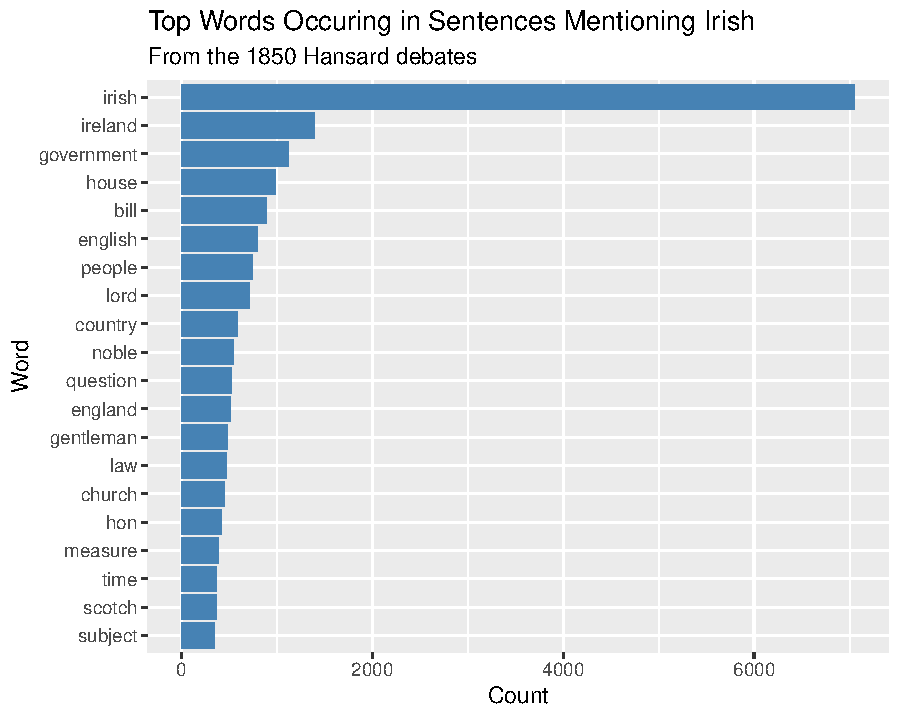
\includegraphics[width=0.8\linewidth]{ch1-11.25.2024_files/figure-latex/unnamed-chunk-54-1}

In this chapter, we used computational historical thinking as a method
for examining change over time. We integrated historical theory, code,
and artificial intelligence (AI) in a hybrid method of analysis. This
method is co-creative: it brings attention to how data processing
techniques shape historical analysis, while also recognizing that
interpretive insights can lead us to revise our computational approach.
In doing so, it emphasizes the dynamic interplay between computation and
historical interpretation.

In the chapters that follow, we will build on this foundation by
introducing more advanced techniques. We will also critically examine
how AI is used in historical research. A key question we will explore is
whether current AI chatbots can generate meaningful historical
interpretations of 19th-century Parliamentary debates.

While AI offers powerful tools for exploratory analysis, we will also
examine the limitations of using AI chatbots as an approach to
computational text analysis, including the conditions under which they
may produce inaccurate or misleading interpretations of history.

\end{document}
